\documentclass[ngerman]{article}

% Packages
% Was macht das hier?
\usepackage[T1]{fontenc}
% Encoding der Datei (um Umlaute so zu nutzen)
\usepackage[utf8]{inputenc}
% Silbentrennung
\usepackage[ngerman]{babel}
% Für \begin{align} und Konsorten
\usepackage{amsmath}
% Für Sätze
\usepackage{amsthm}
% Für \mathbb und Konsorten
\usepackage{amssymb}
% Um im PDF geile Links zu erzeugen
% Weniger unnütze Fehlermeldungen/Warnungen hoffentlich
\usepackage{silence}
% Für internationalisierte Quotes
\usepackage{csquotes}
% Für Subfigures und Figures (alle)
\usepackage{graphicx}
\usepackage[footnotesize,bf]{caption}
\usepackage{subcaption}
% Links (und autoref)
\usepackage[pdfborder={0 0 0}]{hyperref}
%\def\algorithmautorefname{Algorithmus}
\addto\extrasngerman{
	  \def\algorithmautorefname{Algorithmus}
}

% Beide für Tabellen
\usepackage{array}
\usepackage{booktabs}

% Pseudocode
\usepackage{algorithmicx}
\usepackage{algorithm}
\usepackage{algpseudocode}

% Für URLs in Bibliografie
\usepackage{url}

% Macros
\newcommand{\PimiddyName}[1]{\emph{#1}}
\newcommand{\PimiddyBegriff}[1]{\textbf{#1}}
\newcommand{\PimiddyQuotes}[1]{\enquote{#1}}
\newcommand{\PimiddyFormelText}[1]{\textnormal{#1}}
\newcommand{\PimiddyReell}{\ensuremath{\mathbb{R}}}
\newcommand{\PimiddyGanz}{\ensuremath{\mathbb{Z}}}
\newcommand{\PimiddyNorm}[2]{\left\|#2\right\|_{#1}}
\newcommand{\PimiddyFootnote}[1]{\footnote{#1}}
\newcommand{\PimiddyTodo}[1]{{\tiny \textbf{TODO: #1}}}
\newcommand{\PimiddyEnglisch}[1]{{engl. \emph{#1}}}
\newcommand{\PimiddyTableHeading}[1]{{\textbf{#1}}}
\newcommand{\PimiddyInlineCode}[1]{{\texttt{#1}}}
\newcommand{\PimiddyModulo}{\bmod}

\numberwithin{figure}{section}
\numberwithin{equation}{section}
\numberwithin{table}{section}
\numberwithin{algorithm}{section}

% Operators
\DeclareMathOperator*{\PimiddyGrad}{grad}
\DeclareMathOperator*{\PimiddyDiv}{div}
\DeclareMathOperator*{\PimiddyRot}{rot}
\newcommand{\PimiddyLaplace}{\Delta}
\newcommand{\PimiddyProjection}{\mathbb{P}}
\DeclareMathOperator*{\PimiddyVectorfields}{Vect}
\DeclareMathOperator*{\PimiddyScalarfields}{Scal}

% Theorems
\newtheorem*{PimiddySatz}{Satz}

% For latex+inkscape to work. The eps_tex files use \includegraphics{foo.eps}
% which diesn't find the images unless this is defined
\graphicspath{{images/}}
% Also for latex+inkscape
% Also for general colors, dvipsnames adds more colors
\usepackage[usenames,dvipsnames]{xcolor}

\usepackage{listings}

% Fette Monospacefonts
% bold-extra funzt irgendwie nicht
%\usepackage{bold-extra}
%\usepackage[scale=0.9]{beramono}
\usepackage{pxfonts}

\lstdefinelanguage[OpenCL]{C}[ANSI]{C}
{morekeywords={__kernel,kernel,__local,local,__global,global,
	__constant,constant,__private,private,
	char2,char3,char4,char8,char16,
	uchar2,uchar3,uchar4,uchar8,uchar16,
	short2,short3,short4,short8,short16,
	ushort2,ushort3,ushort4,ushort8,ushort16,
	int2,int3,int4,int8,int16,
	uint,
	uint2,uint3,uint4,uint8,uint16,
	long2,long3,long4,long8,long16,
	ulong2,ulong3,ulong4,ulong8,ulong16,
	float2,float3,float4,float8,float16,
	image2d_t,image3d_t,sampler_t,event_t,
	bool2,bool3,bool4,bool8,bool16,
	half2,half3,half4,half8,half16,
	quad,quad2,quad3,quad4,quad8,quad16,
	complex,imaginary}
}
%\lstset{language=[OpenCL]C,basicstyle=\tiny\ttfamily}
\lstset{
	language=[OpenCL]C,
	basicstyle=\small\ttfamily\mdseries,
	keywordstyle=\ttfamily\bfseries\color{blue},
	commentstyle=\itshape,
	classoffset=1,
	morekeywords={
		abs,abs_diff,acos,acosh,acospi,add_sat,all,any,asin,asinh,asinpi,async_work_group_copy,async_work_group_strided_copy,atan,atan2,atan2pi,atanh,atanpi,atomic_add,atomic_and,atomic_cmpxchg,atomic_dec,atomic_inc,atomic_max,acomit_min,atomic_or,atomic_sub,atomic_xchg,atomic_xor,barrier,bitselect,cbrt,ceil,clamp,clz,copysign,cos,cosh,cospi,cross,degrees,distance,dot,erf,erfc,exp,exp10,exp2,expm1,fabs,fast_distance,fast_length,fast_normalize,fdim,floor,fma,fmax,fmin,fmod,fract,frexp,get_global_id,get_global_size,get_global_offset,get_group_id,get_image_channel_data_type,get_image_channel_order,get_image_depth,get_image_dim,get_image_height,get_image_width,get_local_id,get_local_size,get_num_groups,get_work_dim,hadd,half_cos,half_divide,half_exp,half_exp2,half_exp10,half_log,half_log10,half_log2,half_powr,half_recip,half_rsqrt,half_sin,half_sqrt,half_tan,hypot,ilogb,isequal,isfinite,isgreater,isgreaterequal,isinf,isless,islessequal,islessgreater,isnan,isnormal,isnotequal,isordered,isunordered,ldexp,length,lgamma,lgamma_r,log,log10,log1p,log2,logb,mad,mad_hi,mad_sat,mad24,max,maxmag,minmag,mem_fence,min,mix,modf,mul_hi,mul24,nan,native_cos,native_divide,native_exp,native_exp2,native_exp10,native_log,native_log2,native_log10,native_powr,native_recip,native_rsqrt,native_sin,native_sqrt,native_tan,nextafter,normalize,pow,pown,powr,prefetch,radians,read_imagef,read_imageh,read_imageui,read_mem_fence,remainder,remquo,rhadd,rint,rootn,rotate,round,rsqrt,select,shuffle,shuffle2,sign,signbit,sin,sincos,sinh,sinpi,sqrt,step,smoothstep,sub_sat,tan,tanh,tanpi,tgamma,trunc,upsample,vec_step,wait_group_events,write_imagef,write_imageh,write_imagei,write_imageui,write_mem_fence,convert_float4},
	keywordstyle=\color{BlueViolet}}


\lstset{literate=%
	{Ö}{{\"O}}1
	{Ä}{{\"A}}1
	{Ü}{{\"U}}1
	{ß}{{\ss}}2
	{ü}{{\"u}}1
	{ä}{{\"a}}1
	{ö}{{\"o}}1
}

% This is a package nagging about deprecated stuff
\usepackage{nag}

\begin{document}



\section{Danksagungen}

Hiermit möchte ich allen Personen danken, die mich bei der Erstellung der Arbeit
unterstützt haben:

\begin{itemize}
\item Herrn Prof. Dr. Oliver Vornberger für die Tätigkeit als Erstgutachter und
für die Bereitstellung der interessanten Thematik.
\item Frau Prof. Dr. Sigrid Knust, die sich als Zweitgutachterin zur Verfügung gestellt hat.
\item Frau Jana Lehnfeld und Herrn Henning Wenke für das wertvolle Feedback
während der Verfassung der Arbeit.
\end{itemize}

\section{Zusammenfassung}

Die vorliegende Arbeit entstand in der Arbeitsgruppe Medieninformatik an der Universität Osna
im Bereich Computergrafik und beschäftigt sich mit prozeduraler Modellierung. Kern
der Arbeit ist die Generierung einer Schneedecke, um Wetterverhältnisse anhand
von Wetterdaten naturgetreu darstellen zu können. Dazu wird der Anzatz einer
Repräsentation durch Voxel in einem regelmaßigen Voxelgitter verfolgt. Für die
realistische Verteilung des Schnees sorgt dabei die Simulation zufalligen
Schneefalls sowie ein Stabilitatstest, der die Entstehung unnaturlich hoher
Schneeturme verhindert. Abschließend wird das Voxelgitter unter Verwendung des
sogenannten Marching-Cubes-Algorithmus’ in eine schneeahnliche Oberflache
uberfuhrt.


\tableofcontents

\section{Einleitung}

Die Arbeit befasst sich mit der Modellierung und Entwicklung einer Methode zur
Simulation von Wind, sowie einem Partikelsystem für Schneeflocken. Zu Anfang
soll ein Überblick über die Zielsetzung gegeben werden. Danach folgt eine kurze
Zusammenfassung vorhandener Simulationsmethoden. Hier wird die Entscheidung für
eine der Methoden begründet vorgestellt. Schließlich folgt ein Überblick über
den Aufbau der Arbeit.

\subsection{Motivation}

...

\subsection{Zielsetzung}

...

\subsection{Aufbau}

Obacht, was folgt ist aus dem eigentlich geplanten Kapitel
``Implementierung'' entnommen, daher fehlt noch was am Grundaufbau.

In diesem Kapitel soll auf die Details der Implementierung eingegangen werden. Es
wird zunächst OpenGL eingeführt, was zur Visualisierung eingesetzt wird. Danach
wird OpenCL eingeführt, was für die eigentlichen Berechnungen zuständig ist.

Danach das Verfahren von Stam mittels OpenCL umgesetzt. Als Ausgabe erhält man
ein Schnee-Vektorfeld, was dann weiterverwendet werden kann. Hier wird auch auf
Hindernisse wie Gebäude eingegangen. Dazu gehört das Laden der Hindernisse aus
obj-Dateien sowie die Anzeige mittels OpenGL, sowie die Einspeisung in die
Simulation.

Anschließend wird der fallende Schnee modelliert. Hierzu soll zunächst die
Entstehung von Schnee in der Natur erläutert werden, sowie physikalische
Hindergründe bezüglich fallendem Schnee.

Diese idealen physikalischen Gegebenheiten werden dann in ein einfacheres
Modell transformiert, welches für das Partikelsystem verwendet wird. Zu diesem
Partikelsystem gehört neben der Simulation auch die Visualisierung, für die in
dieser Arbeit Pointsprites verwendet werden.

Im letzten Abschnitt wird schließlich auf die Modellierung der Schneedecke
eingegangen, wobei die Ergebnisse von Manuel Schwarz \cite{Schwarz2012} eine
tragende Rolle spielen. Außerdem werden noch einige weitere
Anwendungsmöglichkeiten der Fluidsimulation wie die Simulation von Rauch
angesprochen.

\section{Mathematische Grundlagen}
\label{sec:mathematics}

Die Berechnungen in dieser Arbeit finden alle im reellen Raum statt, also in den
Vektorräumen $\PimiddyReell^n, n \in \{1,2,3\}$. Die Gleichungen der
Strömungsmechanik benutzen \PimiddyBegriff{Vektorfelder} und
\PimiddyBegriff{Skalarfelder}, daher werden diese Begriffe und die zugehörigen
Operationen zunächst eingeführt.

Die später betrachteten Gleichungen sind allerdings meist gar nicht oder nur sehr
schwer analytisch zu lösen, daher greift man auf numerische Verfahren zurück.
Dafür ist es notwendig, Operationen wie den Gradienten oder die
Divergenz zu \emph{diskretisieren}. Im letzten Teil des Abschnitts
werden verschiedene Arten der Diskretisierung erläutert.

\subsection{Kontinuierliche Felder}

Für eine Funktion $f \colon \PimiddyReell^n \to \PimiddyReell$ bezeichne

\begin{equation}
\frac{\partial f}{\partial x_i}
\end{equation}

die \PimiddyBegriff{partielle Ableitung} nach der $i$-ten Komponente.

Ein \PimiddyBegriff{Vektorfeld} $\vec{u}$ ist eine Abbildung

\begin{equation*}
\vec{u} \colon \PimiddyReell^n \to \PimiddyReell^n,
\end{equation*}

die einem Punkt im Raum einen Pfeil zuordnet. So kann \PimiddyzB{}jedem
Punkt im Raum die Windgeschwindigkeit an diesem Punkt zugeordnet
werden. \autoref{fig:mathematics_vectorfield} zeigt ein solches
Vektorfeld.

$\PimiddyVectorfields(\PimiddyReell^n)$ bezeichne die Menge aller
Vektorfelder. In dieser Arbeit betrachtete Vektorfelder sind stets
differenzierbar.

Analog ist ein \PimiddyBegriff{Skalarfeld} $p$ eine Abbildung

\begin{equation*}
p \colon \PimiddyReell^n \to \PimiddyReell
\end{equation*}

welche einem Punkt im Raum einen skalaren Wert zuordnet. Beispielsweise könnte
für jeden Punkt im Raum die dortige Temperatur in einem Skalarfeld gespeichert
sein (siehe \autoref{fig:mathematics_scalarfield}).
$\PimiddyScalarfields(\PimiddyReell^n)$ bezeichne die Menge aller
Skalarfelder. Auch alle Skalarfelder sind in dieser Arbeit
differenzierbar.

\begin{figure}
	\begin{subfigure}[t]{0.5\textwidth}
		\centering
		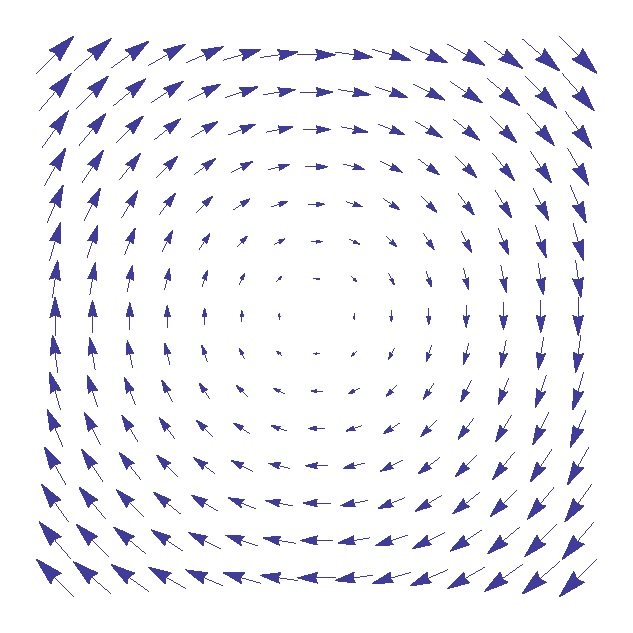
\includegraphics[width=\textwidth]{images/vectorfield}
		\caption{Ein Vektorfeld}
		\label{fig:mathematics_vectorfield}
	\end{subfigure}
	~
	\begin{subfigure}[t]{0.5\textwidth}
		\centering
		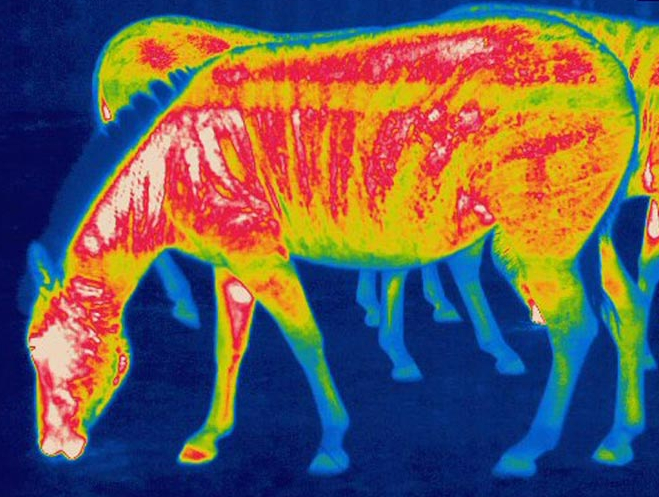
\includegraphics[width=\textwidth]{images/thermal_imaging}
		\caption{Die Körpertemperatur eines Pferds als Skalarfeld.}
		\label{fig:mathematics_scalarfield}
	\end{subfigure}
	\caption{Die betrachteten Feldtypen}
\end{figure}

Sei $p$ ein dreidimensionales Skalarfeld, dann ist der \PimiddyBegriff{Gradient}
$\PimiddyGrad p$ definiert als:

\begin{equation}
\begin{aligned}
\PimiddyGrad \colon \PimiddyScalarfields \to \PimiddyVectorfields \\
\PimiddyGrad p
=
\left( \frac{\partial p}{\partial x},\frac{\partial p}{\partial y},\frac{\partial p}{\partial z} \right)
\end{aligned}
\end{equation}

\begin{figure}[ht]
        \captionsetup{singlelinecheck=off}
	\begin{subfigure}[t]{0.5\textwidth}
		\centering
		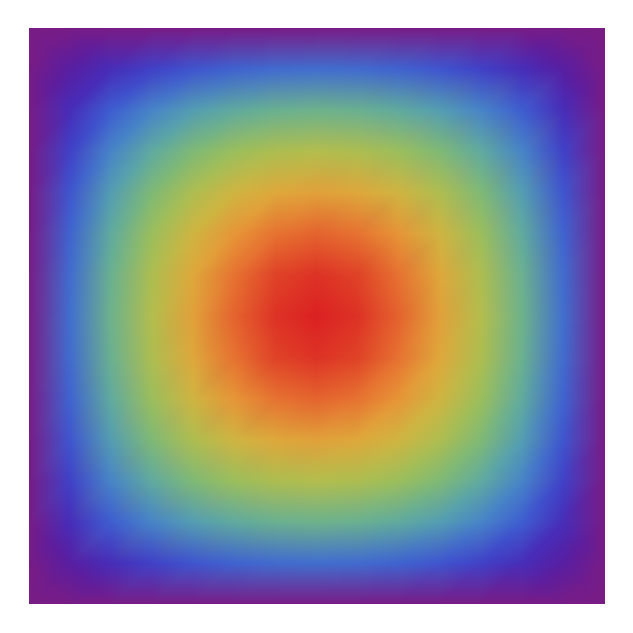
\includegraphics[width=\textwidth]{images/scalar_field_to_show_gradient}
		\caption{Das Skalarfeld zur Funktion \[ f(x,y) = \sin(x)\sin(y) \] Rötliche Färbung deutet hohe Werte an, lila und blau geringe.}
		\label{fig:mathematics_sample_scalar_field}
	\end{subfigure}
	~
	\begin{subfigure}[t]{0.5\textwidth}
		\centering
		
\includegraphics[width=\textwidth]{images/gradient_of_scalar_field}
		\caption{Der Gradient des Skalarfeldes \[ f(x,y)=(\sin(y)\cos(x),\sin(x)\cos(y)) \]}
		\label{fig:mathematics_gradient_of_sample_scalar_field}
	\end{subfigure}
	\caption{Der Gradient am Beispiel}
	\label{fig:mathematics_gradient_of_sample_scalar_field_total}
\end{figure}

Der Gradient eines Skalarfeldes ist also ein Vektorfeld, nämlich das
Vektorfeld der partiellen Ableitungen. Genauso wie die Ableitung eines
Graphen die Steigung an jedem Punkt angibt, so zeigt der Gradient
eines Feldes in die Richtung des steilsten Anstiegs. Die Länge des
Gradienten gibt die Größe der Steigung in diesem Punkt an. Der
Gradient des negativen Skalarfeldes $-p$ zeigt folglich in Richtung
des größten Gefälles.
\autoref{fig:mathematics_gradient_of_sample_scalar_field_total} zeigt
ein simples Beispiel für den Gradienten.

Für differenzierbare Vektorfelder $\vec{u}$ ist die
\PimiddyBegriff{Divergenz} auf dem Feld definiert als

\begin{equation}
\begin{aligned}
\PimiddyDiv \colon \PimiddyVectorfields \to \PimiddyScalarfields \\
\PimiddyDiv \vec{u}
=
\frac{\partial u^x}{\partial x} +
\frac{\partial u^y}{\partial y} +
\frac{\partial u^z}{\partial z}
\end{aligned}
\end{equation}

Hier sind $u^x,u^y,u^z$ die einzelnen Komponenten des Vektorfelds. Die
Divergenz eines Vektorfelds ist also ein Skalarfeld. Dieses Skalarfeld kann
gedeutet werden als \PimiddyQuotes{Quellendichte} des ursprünglichen
Vektorfelds\PimiddyTodo{Hier muss noch ein Bild hin.}. Ein Feld
$\vec{u}$, welches $\PimiddyDiv \vec{u}=0$ erfüllt, heißt folglich
\PimiddyBegriff{quellenfrei}.

In der Physik findet man den Gradienten und die Divergenz meist unter dem Symbol
$\nabla$ vereint. Je nachdem, ob es auf ein Vektor- oder ein Skalarfeld
angewendet wird, wechselt es die Bedeutung.
%Diese Notation wird in der Arbeit bevorzugt, da man die Symbole $\PimiddyGrad$ bzw.\ $\PimiddyDiv$ in der Literatur zu Fluiddynamik kaum vorfindet.

Auf Vektorfeldern ist schließlich die \PimiddyBegriff{Rotation}
definiert als:

\begin{equation}
\begin{aligned}
\PimiddyRot \colon \PimiddyVectorfields \to \PimiddyVectorfields \\
\PimiddyRot \vec{u}
=
\left(
	\begin{array}{c}
		\frac{\partial u^z}{\partial y} - \frac{\partial u^y}{\partial z} \\
		\frac{\partial u^x}{\partial z} - \frac{\partial u^z}{\partial x} \\
		\frac{\partial u^y}{\partial x} - \frac{\partial u^x}{\partial y}
	\end{array}
\right)
\end{aligned}
\end{equation}

Wie der Name schon andeutet gibt sie für jeden Punkt des
ursprünglichen Vektorfelds an, wie stark und in welche Richtung das
Feld in diesem Punkt rotiert. Im Zweidimensionalen ist die Rotation
auch definiert, hier ergibt sich für jeden Punkt im Raum allerdings
nur ein Skalar, kein Vektor. Die Rotationsachse ist immer die
imaginäre \PimiddyQuotes{$z$-Achse} (in
\autoref{fig:mathematics_scalarfield} wäre die Rotation überall
konstant). Ein Feld $\vec{u}$, welches $\PimiddyRot \vec{u}=0$
erfüllt, heißt \PimiddyBegriff{rotationsfrei}.

\begin{figure}
	\begin{subfigure}[b]{0.5\textwidth}
		\centering
		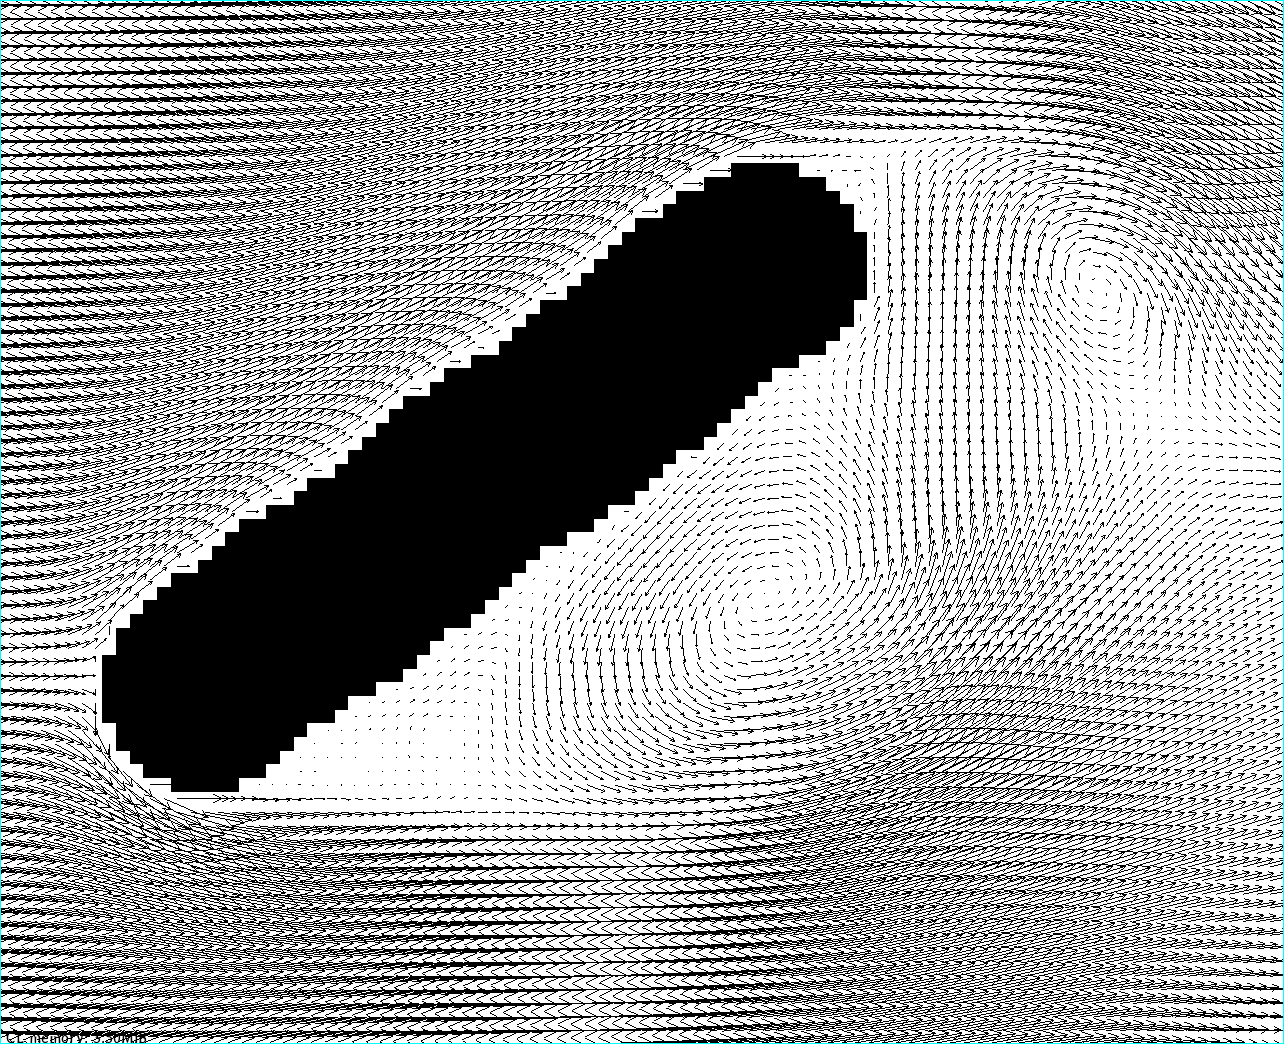
\includegraphics[width=\textwidth]{images/vector_field_rotation_arrows}
		\label{fig:mathematics_image_vectorfield_rotation_arrows}
	\end{subfigure}
	~
	\begin{subfigure}[b]{0.5\textwidth}
		\centering
		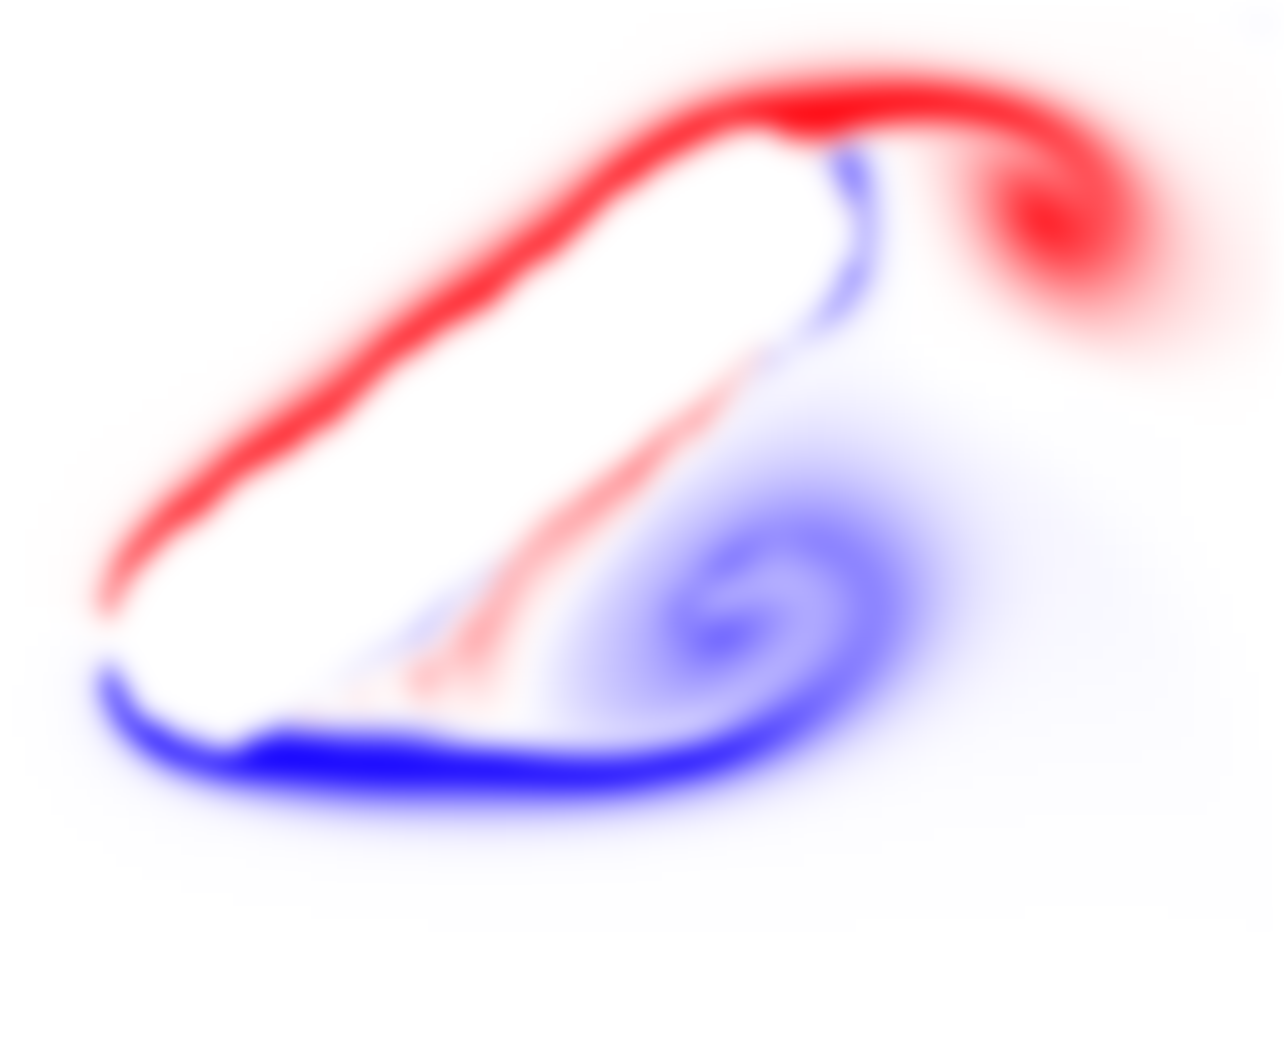
\includegraphics[width=\textwidth]{images/vector_field_rotation}
	\end{subfigure}
	\caption{Ein 2D-Strömungsfeld, das um ein Hindernis herumfließt mit dazugehöriger Rotation. Negative Rotation ist rot gekennzeichnet, positive in blau.}
\end{figure}

Schaltet man $\PimiddyGrad$ und $\PimiddyDiv$ hintereinander, erhält man den
\PimiddyBegriff{Laplace-Operator}:

\begin{equation}
\begin{aligned}
\PimiddyLaplace \colon \PimiddyScalarfields \to \PimiddyScalarfields \\
\PimiddyLaplace p = \PimiddyDiv \PimiddyGrad p
\end{aligned}
\end{equation}

Manchmal wird auch das Symbol $\nabla^2$ für den Laplace-Operator benutzt. Im Dreidimensionalen ergibt sich:

\begin{equation}
\PimiddyLaplace p =
\frac{\partial^2 p}{\partial^2 x} +
\frac{\partial^2 p}{\partial^2 y} +
\frac{\partial^2 p}{\partial^2 z}
\end{equation}

Intuitiv misst der Operator für jeden Punkt $\vec{x}$ die Abweichung von
$p(\vec{x})$ zu Punkten in seiner Umgebung. Die diskretisierte Variante dieses
Operators wird deswegen in der Bildverarbeitung zum Erkennen von Kanten in
Bildern verwendet (siehe \autoref{fig:mathematics_image_laplacian}).

\begin{figure}[ht]
	\begin{subfigure}[t]{0.5\textwidth}
		\centering
		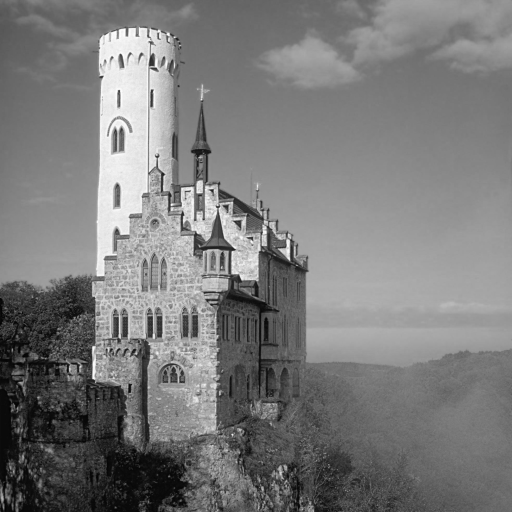
\includegraphics[width=\textwidth]{images/schloss_grey}
		\caption{Originalbild}
	\end{subfigure}
	~
	\begin{subfigure}[t]{0.5\textwidth}
		\centering
		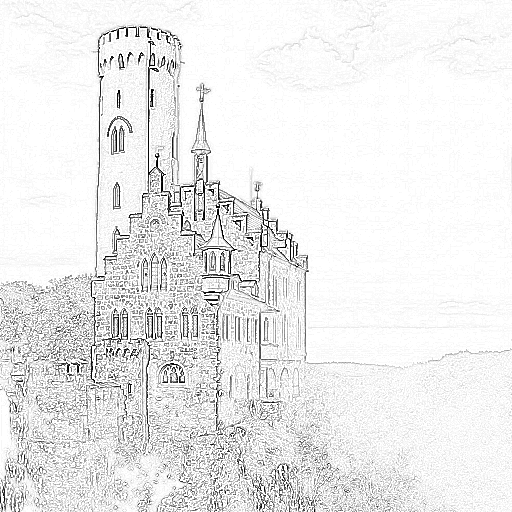
\includegraphics[width=\textwidth]{images/schloss_grey_laplace}
		\caption{Das Bild nach Anwendung des Laplace-Operators}
		\label{fig:mathematics_image_laplacian}
	\end{subfigure}
\end{figure}


Der Operator lässt sich auf nahe liegende Weise auf Vektorfelder erweitern, in drei Dimensionen
ergibt sich:

\begin{equation}
\PimiddyLaplace \vec{u} =
\left(
	\begin{array}{c}
		\PimiddyLaplace u^x \\
		\PimiddyLaplace u^y \\
		\PimiddyLaplace u^z
	\end{array}
\right)
\end{equation}

\subsection{Diskretisierung}
\label{sec:mathematics_discretization}

Die eben vorgestellten mathematischen Definitionen gehen vom
unendlichen, kontinuierlichen Raum $\PimiddyReell^n$ aus. Für die
Berechnungen wird aber ein endliches, diskretes Gitter verwendet, also
eine Teilmenge von $\PimiddyGanz^n$. Eine Zelle in dem diskreten
Gitter wird auch \PimiddyBegriff{Voxel} (für
\PimiddyQuotes{Volumen-Pixel}) genannt. Die eben vorgestellten
Operatoren müssen in eine diskrete Form gebracht werden. Dies wird
hier zunächst in einer Dimension erläutert.

Es sei $f \colon \PimiddyReell \to \PimiddyReell$ eine reelle Funktion, von der
wir in den späteren Berechnungen nur Stützpunkte in regelmäßigen Abständen
$\Delta x$ gegeben haben:

\begin{equation}
f_i = f(x_i) \quad , x_i = n \cdot \Delta x, n \in \PimiddyGanz
\end{equation}

Die (kontinuierliche) Ableitung dieser Funktion ist definiert als

\begin{equation}
f'(x) = \lim_{h \to 0} \frac{f(x) - f(x+h)}{x - h}
\end{equation}

Je nachdem, wie genau die Simulation sein soll, kann bei der
Diskretisierung dieser Ableitung unterschiedlich viel Aufwand
einfließen. Grundlage für die Diskretisierung und die anschließende
Abschätzung der Genauigkeit ist die \PimiddyBegriff{Taylorreihe} von
$f$ (um den Entwicklungspunkt $a$):

\begin{equation}
f(x) = f(a) + f'(a)(x-a) + \frac{f''(a)}{2}(x-a)^2 + O(\Delta x^2)
\end{equation}

Nimmt man als Entwicklungspunkt $f(x_i)$ und setzt $x=x_{i+1}$ erhält man die
\PimiddyBegriff{Vorwärtsdifferenz}-Annäherung der Ableitung:

\begin{equation}
\label{eq:mathematics_forward_difference}
f'(x_i) = \frac{f(x_{i+1}) - f(x_i)}{\Delta x} + O(\Delta x)
\end{equation}

Setzt man $a=x_i,x=x_{i-1}$ erhält man analog die
\PimiddyBegriff{Rückwärtsdifferenz}:

\begin{equation}
\label{eq:mathematics_backward_difference}
f'(x_i) = \frac{f(x_i) - f(x_{i-1})}{\Delta x} + O(\Delta x)
\end{equation}

Der Nachteil dieser beiden Näherungen ist, dass sie einseitig sind (entweder
nach links oder rechts ausgerichtet) und linearen Fehler $O(\Delta x)$ haben, da
die Taylorreihe schon nach dem ersten Glied abgeschnitten wird.

Eine bessere Näherung erhält man, wenn man
\autoref{eq:mathematics_backward_difference} von
\autoref{eq:mathematics_forward_difference} subtrahiert:

\begin{equation}
f'(x_i) = \frac{f(x_{i+1}) - f(x_{i-1})}{2 \Delta x} + O(\Delta x^2)
\end{equation}

Diese Näherung wird \PimiddyBegriff{zentrale Differenz} genannt und
hat nur quadratischen Fehler $O(\Delta x^2)$. Man kann dieses Schema
fortführen, um noch bessere Näherung zu erhalten. Dies führt
allerdings dazu, dass eine immer größere Umgebung des aktuellen
Punktes betrachtet werden muss, was in der späteren Implementierung zu
viele Speicherzugriffe verursacht.

Mit Hilfe der zentralen Differenz lässt sich auch eine Näherung für die zweite
Ableitung angeben:

\begin{equation}
f''(x_i)
=
\frac
{
	f(
		x_{i+1}) -
	2 \cdot
	f(
		x_i)
	+
	f(
		x_{i-1})
}
{
	(\Delta x)^2
}
\end{equation}

Da alle Operatoren auf partiellen Ableitungen beruhen, lassen sich nun
diskrete Näherungen für jeden Operator angeben. Dies ist in
\autoref{table:mathematics_discrete_operator_table} für 3 Dimensionen für ein
Skalarfeld $p$ beziehungsweise ein Vektorfeld $\vec{u}$ geschehen.

\begin{table}[ht]
	\caption{Die diskretisierten Feldoperatoren in drei Dimensionen}
	\centering
	\begin{tabular}{@{}cm{10cm}@{}}
		\toprule \\

			\PimiddyTableHeading{Operator}
		&
			\PimiddyTableHeading{Diskretisierung} \\

		\midrule \\
			$\PimiddyGrad p$
		&
			\begin{equation*}
			\frac{1}{2\Delta x}
			\begin{pmatrix}
				p_{i+1,j,k} - p_{i-1,j,k}
			\\
				p_{i,j+1,k} - p_{i,j-1,k}
			\\
				p_{i,j,k+1} - p_{i,j,k-1}
			\end{pmatrix}
			\end{equation*}
		\\
			$\PimiddyDiv \vec{u}$
		&
			\begin{equation*}
			\frac
			{
				u^x_{i+1,j,k} -
				u^x_{i-1,j,k} +
				u^y_{i,j+1,k} -
				u^y_{i,j-1,k} +
				u^z_{i,j,k+1} -
				u^z_{i,j,k-1}
			}
			{
				2\Delta x
			}
			\end{equation*}
		\\
			$\PimiddyLaplace p$
		&
			\begin{equation*}
			\frac
			{
				p_{i+1,j,k} +
				p_{i-1,j,k} +
				p_{i,j+1,k} +
				p_{i,j-1,k} +
				p_{i,j,k+1} +
				p_{i,j-1,k-1} -
				6p_{i,j}
			}
			{
				(\Delta x)^2
			}
			\end{equation*}
		\\
			$\PimiddyRot \vec{u}$
		&
			\begin{equation*}
			\frac{1}{2\Delta x}
			\begin{pmatrix}
				u^z_{i,j+1,k} - u^z_{i,j-1,k} - u^y_{i,j,k+1} + u^y_{i,j,k-1}
			\\
				u^x_{i,j,k+1} - u^x_{i,j,k+1} - u^z_{i+1,j,k} + u^z_{i,j,k-1}
			\\
				u^y_{i+1,j,k} - u^y_{i-1,j,k+1} - u^x_{i,j+1,k} + u^x_{i,j-1,k}
			\end{pmatrix}
			\end{equation*}
		\\
		\bottomrule
	\end{tabular}
	\label{table:mathematics_discrete_operator_table}
\end{table}

\section{Die Navier-Stokes-Gleichungen}
\label{sec:navier_stokes}

\subsection{Fluide}

Die Gleichungen, die im folgenden beschrieben werden, gelten nicht nur
für Gase wie Luft, sondern auch für Flüssigkeiten wie Wasser. Deshalb
wird im Folgenden der Begriff \PimiddyBegriff{Fluid} verwendet,
welcher beide Zustände zusammenfasst. Physikalisch gesehen sind
Fluide Substanzen, die einer beliebig langsamen Scherung keinen
Widerstand entgegensetzen. Dieses Konzept ist allerdings in dieser
Arbeit nicht von Bedeutung.

Welches Modell man für die Bewegung von Fluiden wählt, hängt davon ab,
welche Art von Fluid man modelliert. Bei dickflüssigen Fluiden wie
Honig muss ein Modell gewählt werden, was die Viskosität gut
modelliert. Bei Fluiden mit geringer Dichte wie Luft können dagegen
einige Faktoren ausgelassen werden. Auch die äußeren Gegebenheiten
haben Einfluss auf das Modell. Daher sollen zunächst die
Rahmenbedingungen des Modells erläutert werden, bevor die zugehörigen
Gleichungen vorgestellt werden.

Das \emph{Volumen} von Fluiden ist im Allgemeinen nicht konstant, es
wird durch Veränderung von Druck und Dichte beeinflusst. Dies
geschieht z.\,B.\ beim Übertreten der Schallmauer (im Medium Luft,
beispielsweise bei einer Explosion) oder bei der Ausbreitung von Tönen
unter Wasser. In der Strömungsmechanik unterscheidet man daher
zwischen \PimiddyBegriff{komprimierbaren} und
\PimiddyBegriff{unkomprimierbaren} Fluiden, je nachdem, ob die
Veränderung des Volumens eine Rolle für die Simulation spielt.

Es werden hier nur \emph{unkomprimierbare} Fluide betrachtet. Dies
stellt kein Problem dar, da nur vergleichsweise kleine
Geschwindigkeiten betrachtet werden.  Das Modell wird dadurch
allerdings wesentlich vereinfacht.

Zudem haben Fluide im allgemeinen an jedem Punkt $\vec{x}$ eine
unterschiedliche \emph{Dichte} $\rho(\vec{x})$. Diese wird im
Wesentlichen von Druck und Temperatur beeinflusst. Zur weiteren
Vereinfachung wird hier allerdings von einer konstanten Dichte $\rho$
ausgegangen und beispielsweise die Temperatur nicht in die
Betrachtungen einbezogen. Effekte wie Auftrieb durch
Temperaturunterschiede können allerdings optional in das Modell
eingepasst werden, siehe \autoref{sec:stam_buoyancy}.

\subsection{Einführung}

Das Modell eines Fluids besteht mathematisch gesehen aus mehreren Feldern
(Skalar- und Vektorfeldern), die den Zustand des Fluids zu einem
\emph{Zeitpunkt} $t$ an einer \emph{Position} $\vec{x}$ angeben.

In den \PimiddyBegriff{Navier-Stokes-Gleichungen}, die in
\autoref{eq:navier_stokes_equation} dargestellt sind, werden zwei
Felder betrachtet, die \emph{Bewegungsgeschwindigkeit}
$\vec{u}(\vec{x},t)$ des Fluids und der \emph{Druck}
$p(\vec{x},t)$. Die Gleichungen wurden 1822 von
\PimiddyName{Claude-Louis Navier} und 1845 von \PimiddyName{George
Gabriel Stokes} formuliert\cite{Muller2003}.

\begin{figure}
\begin{align}
\label{eq:navier_stokes_momentum_equation}
\frac{
	\partial
	\vec{u}
}
{
	\partial t
} +
\vec{u} \PimiddyDiv \vec{u}
& =
\vec{g} +
\nu \PimiddyLaplace \vec{u} -
\frac{
	1
}
{
	\rho
}
\PimiddyGrad p
\\
\label{eq:navier_stokes_incompressibility_condition}
\PimiddyDiv \vec{u} & = 0
\end{align}
\caption{Die unkomprimierbaren Navier-Stokes-Gleichungen}
\label{eq:navier_stokes_equation}
\end{figure}

\autoref{eq:navier_stokes_momentum_equation} ist eine Differentialgleichung, die
wegen des Terms $\vec{u} \PimiddyDiv \vec{u}$ nichtlinear ist. Das macht sie
besonders schwer mit klassischen Verfahren lösbar.

Die Dimension des Raums taucht in den Gleichungen nicht auf, man kann sie also
in zwei oder drei Dimensionen betrachten. Zur Veranschaulichung wird im
Folgenden oft von zwei Dimensionen ausgegangen.

Die einzelnen Bestandteile werden in den folgenden Kapiteln genauer beleuchtet,
hier soll allerdings schon ein kurzer Überblick gegeben werden:

\begin{itemize}
\item
	Die Konstante $\rho$ gibt die \emph{Dichte} des Fluids an. Für Wasser beträgt
	sie etwa $1000 \frac{kg}{m^3}$, für Luft etwa $1.3
        \frac{kg}{m^3}$ \cite{Bridson2007}.
\item
	Der \emph{Druck} $p$ spielt bei den späteren Berechnungen eine große Rolle.
	Er ist dort besonders hoch, wo das Fluid auf Hindernisse
        trifft und diese umfließt.
\item
	Kräfte, die von außen auf das Fluid wirken, wie z.\,B.\ die Schwerkraft
	oder auch der eingeführte Wind, werden im Vektorfeld $\vec{g} \colon
	\PimiddyReell^3 \to \PimiddyReell^3$ zusammengefasst.
\item
	Fluide unterscheiden sich in ihrer \PimiddyBegriff{Viskosität}
	oder \PimiddyQuotes{Zähflüssigkeit}, die in der Gleichung mit $\nu$
	bezeichnet ist. Dickflüssige Fluide wie Honig haben ein hohes $\nu$,
	dünnflüssige wie Luft ein niedriges $\nu$.
\end{itemize}

\autoref{eq:navier_stokes_momentum_equation} wird
\PimiddyBegriff{Impulsgleichung} genannt,
\autoref{eq:navier_stokes_incompressibility_condition} nennt man
\PimiddyBegriff{Unkomprimierbarkeitsbedingung}. Der Name und die Bedeutung der
Gleichungen werden im Folgenden näher beleuchtet.

Die Navier-Stokes-Gleichungen komplett zu erläutern geht über den Rahmen dieser
Arbeit weit hinaus, daher soll vor allem ein intuitives Verständnis der
einzelnen Bestandteile gegeben werden. Außerdem soll eine Beziehung zur
klassischen Mechanik hergestellt werden, da die Gleichungen starke Parallelen
hierzu aufweisen.

\subsection{Die Impulsgleichung}

\subsubsection{Lagrange und Euler}

Um Fluide zu modellieren, gibt es zwei Betrachtungsweisen. Die
\PimiddyBegriff{Euler'sche-Be\-trach\-tungs\-wei\-se} und die
\PimiddyBegriff{Lagrange'sche-Betrachtungsweise}.

Bei der \emph{Lagrange'schen-Betrachtungsweise} modelliert man das
Fluid als System von mikroskopisch kleinen \emph{Partikeln} (man
modelliert sozusagen die Moleküle des Fluids einzeln). Jedes Partikel
hat ein Volumen $V$, eine Masse $m$, eine Position $\vec{x}$ und eine
Geschwindigkeit $\vec{u}$. In jedem Simulationsschritt berechnet man
die Kräfte, die auf die Partikel wirken, und berechnet die
resultierende Beschleunigung mit der Newton'schen Formel:

\begin{align*}
m \cdot \vec{a} &= \vec{F} \\
m \cdot \frac{\partial \vec{u}}{\partial t} &= \vec{F}
\end{align*}

Diese Vorgehensweise ist intuitiv und einfach umzusetzen, aber mathematisch
schwer zu analysieren. Beispielsweise kann man die Frage \PimiddyQuotes{Welche
Geschwindigkeit hat das Fluid an Position $\vec{x}$?} nicht sofort
beantworten. Bei der Bewegung der Schneeflocken ist dies aber äußerst
wichtig.

Bei der \emph{Euler'schen-Betrachtungsweise} hingegen hält man jeweils einen Punkt im
Raum fest und analysiert das Strömungsverhalten (Geschwindigkeit, Temperatur)
durch diesen Punkt. Diese Art der Modellierung ist weniger intuitiv, lässt sich
mit Hilfe von Vektorfeldern und Skalarfeldern aber sehr gut mathematisch erfassen.

\subsubsection{Die substantielle Ableitung}

\begin{figure}[ht]
\centering
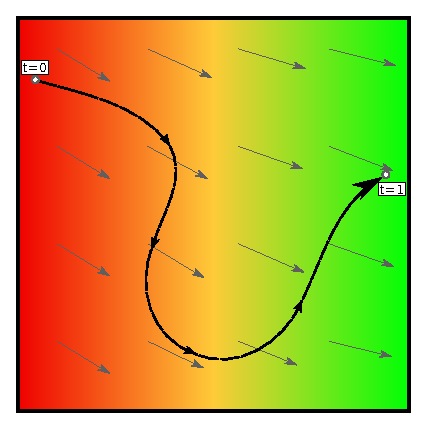
\includegraphics[width=8cm]{images/swimmer_in_water}
\caption{Die Bahn eines Bootes im Wasser. Die Temperatur des Fluids ist hier durch Farben kodiert. Rot bedeutet warmes Wasser, grün bedeutet kaltes Wasser. Nicht dargestellt ist die Veränderung der Wassertemperatur über die Zeit.}
\end{figure}

Sowohl die Euler'sche- als auch die Lagrang'sche Betrachtungsweise spiegeln sich
in den Navier-Stokes-Gleichungen wider. Obwohl es nicht sofort
erkennbar ist, bilden die Gleichungen eine Entsprechung der Gleichung
$\vec{F} = m \cdot \vec{a}$ mit dem Unterschied, dass keine Kraft auf
einen einzelnen Körper berechnet wird, sondern auf einen ganzen
Raumabschnitt (ein \PimiddyQuotes{Kontinuum}).

Was die beiden Betrachtungsweisen verbindet, ist die
\PimiddyBegriff{substantielle Ableitung}. Zur Herleitung dieser
Ableitungsform betrachten wir zunächst eine beliebige Größe
$q(\vec{x},t)$. Dies kann eine skalare Größe wie z.\,B.\ die Temperatur
eines Gewässers sein oder eine Vektorgröße wie die Farbe des Wassers
an einem Punkt. Da $q$ in jedem Punkt definiert ist, stellt die
Funktion eine Euler'sche Größe dar.

Zudem betrachten wir ein Partikel mit einer Bewegungsbahn durch das
Fluid (z.\,B.\  ein Ruderboot im Wasser). Seine Position zum Zeitpunkt
$t$ sei gegeben durch $\vec{p}(t)$. Dies entspricht einer
Lagrange'schen Größe.

Setzen wir beide Größen zusammen, erhalten wir beispielsweise die
Temperatur des Wassers auf der Bahn, die das Boot im Wasser verfolgt:

\begin{equation}
\PimiddyFormelText{Temperatur}(t) = q(\vec{p}(t),t)
\end{equation}

Wollen wir wissen, wie sich die Umgebungstemperatur des Bootes im Lauf
der Zeit verändert, bilden wir die (totale) Ableitung dieser
zusammengesetzten Größe:

\begin{equation}
\frac{
	\partial \PimiddyFormelText{Temperatur}(t)
}
{
	\partial t
}
=
\frac{
	\partial q
}
{
	\partial t
}
+
\PimiddyGrad q \cdot
\frac{
	\partial \vec{p}}
{
	\partial t
}
\end{equation}

Die Summe auf der rechten Seite besteht aus zwei Teilen. Der erste Term,
$\frac{\partial q}{\partial t}$, gibt an, wie sich das Fluid unabhängig von
der betrachteten Position verändert. Bezogen auf das Boot gibt dieser
Term an, wie sich die Temperatur des Gewässers über den Tag verteilt
verändert, beispielsweise durch den Einfluss der Sonnenstrahlen. Der
zweite Term ergänzt die globale Ableitung durch die lokale
Temperaturänderung, die durch die Bahn des Bootes verursacht
wird.

Statt eines beliebigen Pfades durch das Fluid nimmt man zur Definition der
substantiellen Ableitung nun das Geschwindigkeitsfeld des Fluids zur Hilfe:

\begin{equation}
\frac{
	Dq}
{
	Dt
} :=
\frac{
	\partial q
}
{
	\partial t
}
+
\PimiddyGrad q \cdot
\vec{u}
\end{equation}

Man geht also von einem Partikel aus, was sich im Fluid \PimiddyQuotes{treiben}
lässt, und misst die Veränderung der Größe $q$ auf seiner Bahn. Analog ist die
substantielle Ableitung für Vektorgrößen definiert:

\begin{equation}
\frac{
	D\vec{q}}
{
	Dt
} :=
\frac{
	\partial q
}
{
	\partial t
}
+
\PimiddyDiv q \cdot
\vec{u}
\end{equation}

Die Impulsgleichung lässt sich mit Hilfe der substantiellen Ableitung so schreiben:

\begin{equation}
\rho \frac{D\vec{u}}{Dt} = - \PimiddyGrad p + \PimiddyLaplace \vec{u} + \vec{f}
\end{equation}

Dies entspricht der klassischen Newton'schen Kraftformel, wobei die
Masse $m$ durch die Dichte $\rho$ ersetzt wird. Auf der rechten Seite
der Gleichung stehen die Kräfte, die das Fluid beeinflussen. Diese
Kräfte sollen im Einzelnen näher beschrieben werden.

\subsubsection{Die Kräfte in den Navier-Stokes-Gleichungen}

Die Kraft, die überall im Fluid in gleicher Weise wirkt, ist die Schwerkraft:

\begin{equation}
F_g =
\left(
\begin{array}{c}
0 \\
-g \\
0
\end{array}
\right)
\end{equation}

mit $g \cong 9.81 \frac{m}{s^2}$.

Durch den Druck $p$ des Fluids wird eine weitere Kraft $F_p$ ausgeübt.
Allerdings erzeugt die Anwesenheit von Druck (also $p \neq 0$) allein
keine Kraft. Ist der Druck beispielsweise im gesamten Fluid konstant,
ist die ausgeübte Kraft gleich 0. Stattdessen wirkt $F_p$
\PimiddyQuotes{ausgleichend}. Sie zeigt von Bereichen hohen Drucks hin
zu Bereichen niedrigeren Drucks. Mathematisch gesehen ist $F_p$ also
proportional zum negativen Gradient des Drucks.

\begin{equation}
\label{eq:navier_stokes_f_p}
F_p = -\PimiddyGrad p
\end{equation}

 In \autoref{fig:navier_stokes_particle_system_wall_collision}) ist
dies intuitiv anhand eines Partikelsystems erläutert. Treffen die
Partikel auf eine Wand, entsteht Druck, der tangential zur Wand wirkt
und die Partikel in diese Richtung beschleunigt. In den späteren
Berechnungen spielt der Druck insbesondere eine Rolle, um das Fluid in
seinem unkomprimierbaren Zustand zu halten und um das Hineinfließen in
Hindernisse zu verhindern.

\begin{figure}[ht]
\centering
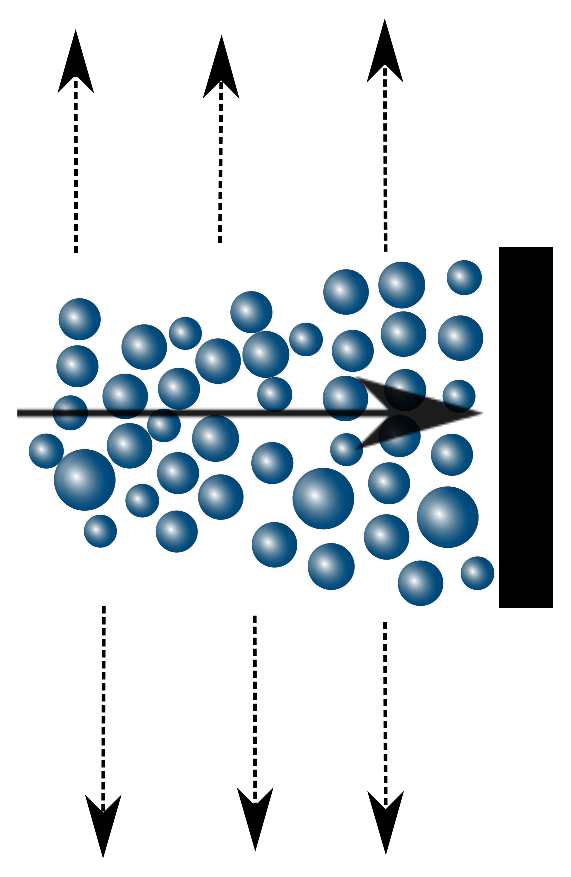
\includegraphics[width=6cm]{images/particle_system_wall_collision}
\caption{Partikelsystem, das auf ein Hindernis prallt. Der durchgezogene Pfeil deutet die Fließrichtung an, die gestrichelten Pfeile den negativen Gradienten des Drucks. Die Partikel erfahren also eine Kraft nach außen.}
\label{fig:navier_stokes_particle_system_wall_collision}
\end{figure}

Die Viskosität des Fluids hat ebenfalls Einfluss auf das Fluid. Bei einem
viskosen Fluid wird jeder Deformation ein Widerstand entgegengesetzt. Eine
Flüssigkeit wie Honig, die um ein Hindernis herumfließt, bildet hinter dem
Hindernis keine Verwirbelungen; die hohe Viskosität wirkt dem entgegen. Luft
hingegen hat eine niedrige Viskosität, bildet also besonders viele Wirbel.

Die Kraft, die durch die Viskosität ausgeübt wird, hat den Effekt,
Geschwindigkeitsunterschiede innerhalb des Fluids auszugleichen. Sie ist
daher proportional zum Laplace der Geschwindigkeit:

\begin{equation}
\label{eq:navier_stokes_f_v}
F_v = \mu \cdot \PimiddyLaplace \vec{u}
\end{equation}

Die Konstante $\mu$ stellt die \PimiddyBegriff{dynamische Viskosität}
des Fluids dar.

\subsection{Die Unkomprimierbarkeitsbedingung}
\label{sec:mathematics_incompressibility_condition_section}

\begin{figure}[ht]
\centering
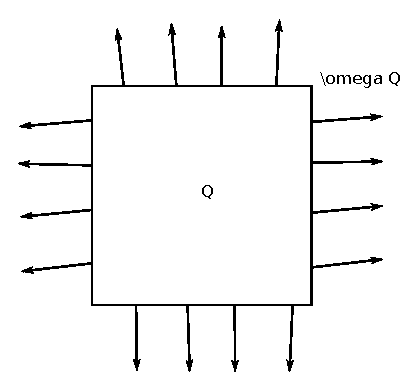
\includegraphics[width=10cm]{images/incompressibility_condition_example}
\caption{Fluss durch ein Rechteck. Der große Pfeil deutet die Fließrichtung des Fluids an. Die Pfeile an den Rändern des Rechtecks zeigen in die dortige Fließgeschwindigkeit, über deren Normalenkomponente in \autoref{eq:navier_stokes_incompressibility_initial_integral} integriert wird.}
\label{fig:navier_stokes_incompressibility_condition_example}
\end{figure}

Um die Unkomprimierbarkeitsbedingung zu motivieren, sei ein beliebiges Volumen
$\Omega \subset \PimiddyReell^3$ gegeben, \PimiddyzB ein Würfel im Raum. Seine
Oberfläche sei $\partial \Omega$.

Die Änderung des Würfelvolumens über die Zeit kann berechnet werden,
indem man über die Normalenkomponente entlang seiner Oberfläche
integriert \cite{Chorin1980}. Bildlich gesprochen summiert man auf
diese Weise eingehende und ausgehende Strömungen an den
Würfelseitenflächen (\Pimiddyvgl
\autoref{fig:navier_stokes_incompressibility_condition_example}):
\begin{equation}
\label{eq:navier_stokes_incompressibility_initial_integral}
\frac{
	\partial \PimiddyFormelText{Volumen}(\Omega)
}
{
	\partial t
}
=
\iint_{\partial \Omega} \vec{u} \cdot \vec{n}
\end{equation}
Damit die Flüssigkeit unkomprimierbar ist -- sich das Volumen also
nicht ändert -- sollte dieses Integral verschwinden:
\begin{equation}
\iint_{\partial \Omega} \vec{u} \cdot \vec{n} = 0
\end{equation}
Mit Hilfe des Divergenzsatzes können wir dieses Integral in ein Volumenintegral
umformen:
\begin{equation}
\iiint_\Omega \PimiddyDiv \vec{u} = 0
\end{equation}
Da $\Omega$ beliebig gewählt war, folgt die
Unkomprimierbarkeitsbedingung $\PimiddyDiv \vec{u} = 0$.

\section{Methode nach Stam}

\subsection{Motivation}

Die Methode zur approximativen Lösung der Navier-Stokes-Gleichungen, die im
Folgenden erklärt wird, wurde von \PimiddyName{Jos Stam} im Jahr 1999 entwickelt
und in dem Paper "`Stable Fluids"' vorgestellt \cite{Stam1999}. Das Verfahren
wurde speziell für die Computergrafik entwickelt, wobei auf einige
Besonderheiten eingegangen wurde:

\begin{enumerate}
\item
	Im Gegensatz zu wissenschaftlichen Simulationen ist man in der
	Computergrafik an einer Lösung interessiert, die in möglichst kurzen
	Abständen Ergebnisse produziert. Zum Beispiel möchte man die
	Strömungssimulation jedes Frame um einen Zeitschritt weiterbewegen. Um
	eine flüssige Simulation zu erhalten, ist die Laufzeit des
	Lösungsalgorithmus also auf 16 Millisekunden (für 60 Bilder pro Sekunde)
	bzw. 33 Millisekunden (für 30 Bilder pro Sekunde) beschränkt. Die
	Navier-Stokes-Gleichungen bilden als System von nichtlinearen
	Differentialgleichungen hier eine besondere Herausforderung.
\item
	Man ist außerdem nicht unbedingt an einer exakten Lösung interessiert.
	Will man z.\,B. Wasser oder Rauch simulieren reicht es, ein physikalisch
	annähernd korrektes Verhalten zu erzielen.
\item
	Bisherige Verfahren (wie z.\,B. die finiten Differenzen in
	\cite{Foster1997}) waren numerisch \emph{instabil} für große
	Zeitschritte. Dynamische Anwendungen wie Spiele oder Animationssoftware
	können allerdings keine minimiale Framerate garantieren, da sie mit
	verschiedenen Umgebungen und Hardwarekonfigurationen ausgeführt werden
	können.

	Als Ausweg muss man einen großen Zeitschritt (ein langes Frame) entweder
	ignorieren -- was die Simulation unrealistisch macht -- oder ihn in
	kleinere Zeitschritte unterteilen. Die Laufzeit des Verfahrens ist aber
	im Allgemeinen nicht von der Größe des Zeitschritts abhängig. Dies führt
	dazu, dass das nächste Frame erneut viel Rechenzeit benötigt und wieder
	entsprechend lang wird.

	Dieser Effekt ist nicht mehr aufzuhalten und die Simulation
	\PimiddyQuotes{explodiert}.
\item
	Bisherige Verfahren waren auf Hilfe des Designers angewiesen, um Teile
	der Simulation möglichst realistisch zu modellieren. Bestimmte natürlich
	vorkommende Turbulenzen mussten explizit in die Simulation eingegeben
	werden. Idealerweise sollte die Simulation allerdings von selber
	fortgeführt werden, der Designer sollte nur Rahmenbedingungen wie
	Hindernisse und globale Eigenschaften des Fluids (wie Dichte und
	Viskosität) vorgeben.
\end{enumerate}

\begin{figure}[ht]
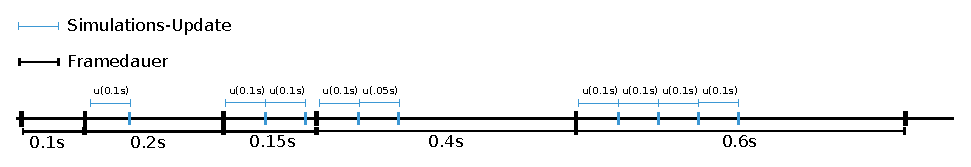
\includegraphics[width=12cm]{images/simulation_blowup}
\caption{Instabilität in Simulationen: Hier wird angenommen, die maximal zu simulierende Simulationsdauer sei $0.1s$. Längere Frames werden in mehreren Ticks berechnet, die aber konstant lange Laufzeit haben. Dies führt zu dauerhaft langen Frames, der Effekt potenziert sich.}
\end{figure}

Das Verfahren ist also auf Geschwindigkeit ausgelegt, basiert aber
nichtsdestotrotz auf den Navier-Stokes-Gleichungen und erzielt akkurate
Simulationsergebnisse. Anfängliche Schwachstellen des Verfahrens wie die zu
starke Dämpfung von Wirbeln wurden in weiteren Arbeiten ausgebessert
\cite{Foster}. Diese Verbesserungen sind teilweise auch in die Arbeit
eingeflossen.

Wegen der numerischen Stabilität und sehr guten Parallelisierbarkeit wird Stams
Verfahren bereits in einigen Spielen eingesetzt (siehe \cite{Crane2007},
\cite{Peschel2009}). Hier beschrieben wird eine leicht abgewandelte
Fassung, bei der andere Randbedingungen verwendet werden.

\subsection{Überblick über das Verfahren}

Die Fluidsimulation findet auf einem diskreten, endlichen Gitter, also einer
Teilmenge von $\PimiddyGanz^n$ statt. Gegeben sei das Geschwindigkeitsfeld zum
Zeitpunkt $t$: $\vec{u}_{i,j,k}^t$. Als Anfangsbedingung könnten zum Zeitpunkt $0$
z.\,B. alle Zellen auf eine vorgegebene \PimiddyQuotes{Windrichtung} gesetzt sein.
Gegeben sei außerdem ein Zeitdelta $\Delta t$ (nicht zu verwechseln mit dem
Laplaceoperator). Ziel ist es, unter Zuhilfenahme der
Navier-Stokes-Gleichungen ein neues Geschwindigkeitsfeld $\vec{u}_{i,j,k}^{t+\Delta
t}$ zu berechnen.

Außerdem berechnen wir einmalig ein \emph{Hindernisfeld} $b_{i,j,k}$. Ist $b_{i,j,k}
= 1$, dann ist diese Zelle mit einem Hindernis ausgefüllt. Ist $b_{i,j,k} = 0$,
ist die Zelle frei. Im Implementierungsteil wird erklärt, wie dieses
Hindernisfeld gefüllt wird.

Die rechte Seite der Impulsgleichung \eqref{eq:navier_stokes_momentum_equation} besteht
aus mehreren Summanden:

\begin{equation}
\vec{u} \PimiddyDiv \vec{u} -
\nu \PimiddyLaplace \vec{u} +
\vec{g} -
\frac{
	1
}
{
	\rho
}
\PimiddyGrad p
\end{equation}

In Stams Verfahren wird jeder dieser Summanden als eine Operation betrachtet,
die ein Geschwindigkeitsfeld sowie eventuell weitere Eingabegrößen wie $\Delta
t$ erhält, und die ein neues Geschwindigkeitsfeld zurückgibt. Das so berechnete
neue Feld wird zur Eingabe der darauffolgenden Operation. So wird die Lösung der
Impulsgleichung in kleinere Teile zerlegt, die für sich behandelt werden können:

\begin{itemize}
\item
	Der Term
	\begin{equation}
	\vec{u} \PimiddyDiv \vec{u}
	\end{equation}
	stellt die \PimiddyBegriff{Advektion} dar. Das Vektorfeld wird entlang
	seiner eigenen Strömungsrichtung weiterbewegt. Er sei im Folgenden mit
	\PimiddyInlineCode{advection}$(\vec{u},\Delta t)$ bezeichnet.
\item
	Der Term
	\begin{equation}
	\nu \PimiddyLaplace \vec{u}
	\end{equation}
	stellt die viskose \PimiddyBegriff{Diffusion} dar. Selbst wenn keine
	Kräfte auf das Fluid wirken, bewegt es sich durch Diffusionsprozesse
	weiter, so wie Farbe auf einem Blatt Papier verläuft.

	Dieser Term kann in Stams Verfahren ignoriert werden. Diffusion entsteht
	ohnehin \PimiddyQuotes{zufällig} durch Genauigkeitsfehler während der
	Advektion (siehe unten). So kann Performance eingespart werden, denn die
	Lösung dieses Terms ist sehr aufwändig.
\item
	Der Term $\vec{g}$ umfasst schlicht das Aufsummieren aller äußeren
	Kräfte, die auf das Fluid wirken. Hierzu gehört sowohl die Schwerkraft
	als auch der von außen eingeführte Wind. Die Operation bekommt als
	Eingabe das Geschwindigkeitsfeld sowie das Zeitdelta (bei größerem
	Zeitunterschied zum letzten Simulationsschritt sollen die Kräfte
	stärker wirken). Sei sei im folgenden mit
	\PimiddyInlineCode{externalForces}$(\vec{u},\Delta t)$ bezeichnet.
\item
	Der \emph{Druck} des Fluids wird in dem Term
	\begin{equation}
	-\frac{1}{\rho} \PimiddyGrad p
	\end{equation}
	zusammengefasst. Er dient am Ende unter anderem dazu, die
	Randbedingungen und die Un"-komp"-ri"-mier"-bar"-keit zu erzwingen. Die Berechnung
	des Drucks sei mit \PimiddyInlineCode{calculatePressure}$(\vec{u})$
	bezeichnet.
\item
	Wie bei Differentialgleichungen üblich, müssen wir noch die
	\emph{Rand- und Anfangsbedingungen} behandeln. Dadurch wird
	einerseits sichergestellt, dass der das Fluid nicht in Hindernisse
	eindringt, andererseits an den Rändern der Simulation frei hinausfließen
	kann. Diese Operation wird im Folgenden als
	\PimiddyInlineCode{boundaries}$(\vec{u})$ bezeichnet und wird vor der
	Berechnung des Drucks eingefügt.
\end{itemize}

\begin{algorithm}
\caption{Der Lösungsalgorithmus in Pseudocode}
\label{alg:stam_first_algorithm}
\begin{algorithmic}
\Function{simulate}{$\vec{u}$,$\Delta t$}
	\State $\vec{u}'$ = advection($\vec{u}$,$\Delta t$)
	\State $\vec{u}''$ = externalForces($\vec{u}'$,$\Delta t$)
	\State $\vec{u}'''$ = boundaries($\vec{u}''$)
	\State $p$ = calculatePressure($\vec{u}$)
	\State \Return $\vec{u}''' - \PimiddyGrad p$
\EndFunction
\end{algorithmic}
\end{algorithm}

\begin{figure}[ht]
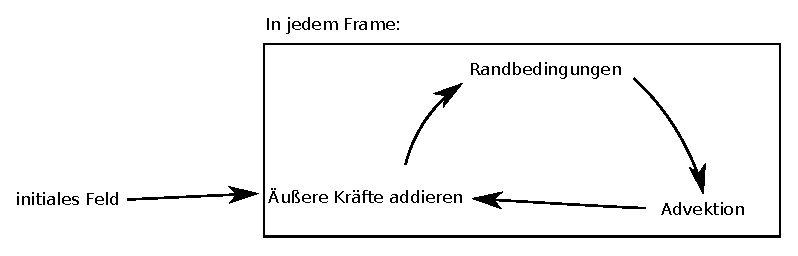
\includegraphics[width=10cm]{images/stam_loop}
\caption{Die Simulationsschleife ohne Projektion.}
\end{figure}

Für jeden Term wird im Folgenden ein Lösungsalgorithmus vorgestellt, insgesamt
erhält man den Pseudocode in \autoref{alg:stam_first_algorithm}.

\subsection{Advektion}

Wie bereits in der Erklärung der Navier-Stokes-Gleichungen angedeutet, wird bei
der Advektion das Geschwindigkeitsfeld entlang \PimiddyQuotes{sich selber}
weiterbewegt. Auf diese Weise kann sich Wind, der von einer Seite der
Simulation eingeführt wird, über den gesamten Simulationsbereich ausbreiten.
Manchmal spricht man daher auch von \emph{Selbstadvektion}. In älterer Literatur
ist auch von \emph{Konvektion} die Rede.

Im Folgenden gehen wir etwas allgemeiner davon aus, dass eine \emph{beliebige} Größe
$q_{i,j,k}^t$ entlang des Vektorfelds $\vec{u}$ bewegt werden soll. Die Methode
\PimiddyInlineCode{advection} kann also auch verwendet werden, um
Temperaturwerte oder die Dichte des Rauchs an einer Stelle entlang des
Vektorfeldes weiterzubewegen. Als Ausgabe erhalten wir ein neues Feld
$q_{i,j,k}^{t+\Delta t}$.

Um die Advektion durchzuführen gibt es mehrere Ansätze. Der gängigste arbeitet
mit der Methode der finiten Differenzen und wurde unter anderem in
\cite{Foster} benutzt. Finite Differenzen führen aber zu einem numerisch
instabilen Algorithmus. Im Gegensatz dazu soll hier zunächst ein intuitiver
Ansatz erläutert werden, der auch numerisch instabil ist und somit nicht ohne
große Einschränkungen verwendbar ist. Dieser Ansatz wird danach leicht
modifiziert, um Stabilität zu erreichen.

\begin{figure}[ht]
\centering
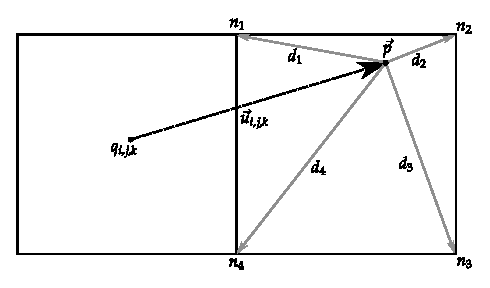
\includegraphics[width=6cm]{images/advection_bad}
\caption{Das numerisch instabile Advektionsverfahren}
\label{fig:stam_numerically_unstable_advection}
\end{figure}

Das neue Feld $q_{i,j,k}^{t+\Delta t}$ sei anfangs überall 0 (bzw\,. $(0,0,0)$,
falls es ein Vektorfeld ist). Man stelle sich an jedem Gitterpunkt
$(i,j,k)$ ein Partikel mit \PimiddyQuotes{Ladung} $q_{i,j,k}$ vor, was im Fluid
treibt. Durch die Bewegung des Fluids würde dieses Partikel um $\Delta t \cdot
\vec{u}_{i,j,k}$ verschoben und läge im nächsten Zeitschritt bei
$\vec{p}=(i,j,k)+\Delta t \cdot \vec{u}_{i,j,k}$. Somit läge es im Allgemeinen
nicht mehr \emph{exakt} auf einem Gitterpunkt, sondern zwischen 8 Nachbarpunkten
$n_i \in \PimiddyGanz^3, i \in \{1,\ldots,8\}$ (siehe
\autoref{fig:stam_numerically_unstable_advection}). Man bestimmt jetzt die
Distanz von $\vec{p}$ zu jedem der Nachbarpunkte:

\begin{equation}
d_i = \PimiddyNorm{2}{\vec{p} - n_i}, i \in \{1,\ldots,8\}
\end{equation}

Diese $d_i$ dienen als Gewichtung, um die \PimiddyQuotes{Ladung} $q_{i,j,k}$
anteilig auf die Nachbarknoten aufzuteilen:

\begin{equation}
q_{n_i}' \leftarrow q_{n_i}' + d_i \cdot q_{i,j,k}
\end{equation}

Dieses Verfahren ist intuitiv und einfach zu implementieren. Aber es ist
numerisch nicht stabil und führt zu Oszillationen (für eine genaue Betrachtung
sei auf die Literatur verwiesen).

Stam wählte einen anderen Ansatz, die sogenannte \emph{Methode der
Charakteristika}. Die Idee ist ähnlich zu der gerade vorgestellten, funktioniert
aber in die \PimiddyQuotes{umgekehrte Richtung}.

\begin{figure}[ht]
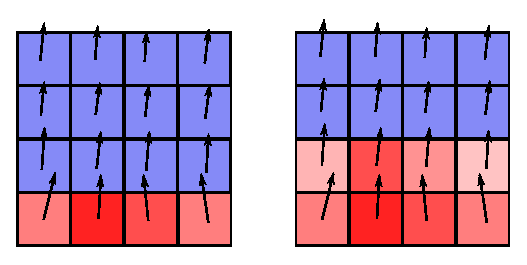
\includegraphics[width=6cm]{images/advection_bad_example}
\caption{Das numerisch instabile Advektionsverfahren für ein Temperaturfeld}
\end{figure}

Man betrachtet wieder jeden Gitterpunkt $(i,j,k)$ einzeln, stellt sich diesmal
allerdings vor, man sei auf der Zeitachse im Punkt $t+\Delta t$, also bereits im
nächsten Zeitschritt. Das (gedachte) Partikel an Position $(i,j,k)$ habe die
Geschwindigkeit $\vec{u}_{i,j,k}^t$.

Rechnet man auf der Zeitachse um $\Delta t$ zurück, erhält man die
\PimiddyQuotes{vorherige} Position des Partikels, nämlich $(i,j,k) - \Delta t
\cdot \vec{u}_{i,j,k}^t$ \PimiddyFootnote{Hier wird nur ein Schritt der
Partikelflugbahn zurückverfolgt. Es besteht die Möglichkeit, mehrere
Schritte zurückzuverfolgen, die ist aber aufwändig zu implementieren.}. Es
ergibt sich allerdings dasselbe Problem wie bei dem vorher beschriebenen Ansatz:
Diese Position liegt nicht genau auf dem Gitter, sondern dazwischen (siehe
\autoref{fig:stam_good_advection}).

Als Lösung \emph{interpolieren} wir zwischen den 8 Nachbarwerten des
verschobenen Partikels und schreiben den entstehenden Wert in die Zelle
$u_{i,j,k}^{t+\Delta t}$. Dies ist eine Operation, auf die Grafikkarten stark
optimiert sind, und bei denen traditionell Texturen hohe Performance erreichen
können.

Allerdings liegt hier auch eine Fehlerquelle des Verfahrens. Interpolation ist
eine glättende Operation, sie liefert nur eine \emph{Approximation} des Wertes,
der zwischen den Gitterzellen angenommen würde. Ähnlich wie bei der
Herleitung der diskreten Ableitung in \autoref{sec:mathematics_discretization}
muss man in der Implementierung einen Kompromiss eingehen und ein
Interpolationsverfahren wählen, was Genauigkeit und Rechenleistung verbindet.

Auch für große Zeitschritte liefert das Verfahren ein Vektorfeld als Ausgabe,
was in seinem Wertebereich beschränkt ist, denn die Interpolation liefert kein
Wert zurück, der betragsmäßig größer ist als die Ausgangswerte. Das Verfahren
ist deshalb stabil. Allerdings sollte $\Delta t$ nicht zu groß gewählt werden.
\cite{Foster} gibt hier als Richtlinie etwa $5\times$ die Gittergröße an.

\begin{figure}[ht]
\centering
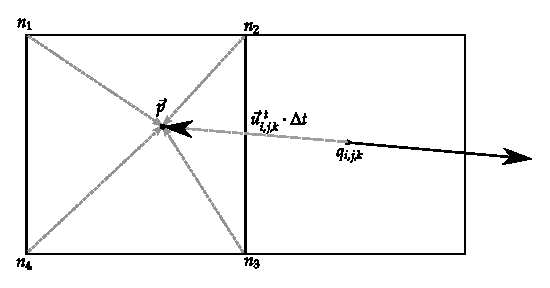
\includegraphics[width=6cm]{images/advection_good}
\caption{Stams stabiles Advektionsverfahren}
\label{fig:stam_good_advection}
\end{figure}

Natürlich kann es passieren, dass wir über den Rand des Simulationsbereiches
\PimiddyQuotes{hinauslaufen}. Es gibt mehrere Möglichkeiten, dies zu behandeln.
Beispielsweise könnte man auf die gegenüberliegenden Seite des
Simulationsbereiches umbrechen (periodische Randbedingung), was in Stams Arbeit
getan wurde. Alternativ kann man die Gerade betrachten, die durch den
Mittelpunkt der aktuellen Zelle geht, und diese Gerade mit den Rändern der
Simulation schneiden. Man wählt dann den Schnittpunkt auf dem Rand als Basis für
die Interpolation (siehe \autoref{fig:stam_clamping_borders}). Dies wurde in der
Arbeit implementiert.

\begin{figure}[ht]
\centering
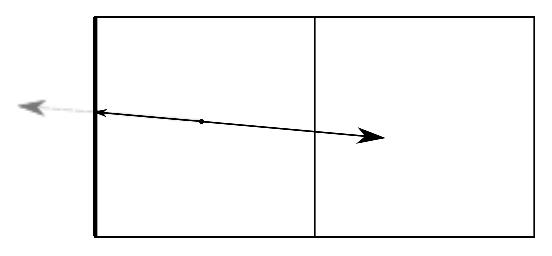
\includegraphics[width=6cm]{images/advection_clamping_borders}
\caption{Abschneiden der Geschwindigkeit an den Rändern}
\label{fig:stam_clamping_borders}
\end{figure}

Weiterhin kann der zurückberechnete Vektor $(i,j,k) - \Delta t u_{i,j,k}^t$ in
einem Hindernis landen. Man kann in diesem Fall einen Geschwindigkeitswert
von $(0,0,0)$ annehmen, was einem stationären Hindernis wie einem Gebäude
entspricht. Es ist aber auch möglich, ein weiteres Vektorfeld
$\vec{u}_{\PimiddyFormelText{boundary}}$ zu verwalten, wo für jede Gitterzelle die
\emph{Geschwindigkeit} des dort vorhandenen Hindernisses notiert ist. Dies wurde
in \cite{Crane2007} umgesetzt. Für die Simulation in dieser Arbeit wurde von
unbeweglichen Hindernissen ausgegangen.

\PimiddyTodo{Hier kurz erklären, dass das auch Semilagrangeadvektion genannt wird.}

\subsection{Äußere Kräfte}

\subsubsection{Gravitation}

Zu den äußeren Kräften gehört zu allererst die \emph{Gravitation}. Diese lässt
sich sehr einfach ausdrücken:

\begin{equation}
F_g = \Delta t (0,-9.81,0)
\end{equation}

\subsubsection{Auftrieb}

\PimiddyTodo{Auftrieb allgemein und konkret mit Buissnesq erklären}

\subsubsection{Wirbelstärkenerhaltung}

Der Advektionsschritt enthält eine lineare Interpolation, um die
Geschwindigkeitswerte in der Nachbarschaft des zurückverfolgten Partikels zu
finden. Diese simple Interpolationsmethode führt allerdings dazu, dass
Genauigkeit bei der Simulation verloren geht. Dadurch werden viele interessante
Phänomene in Fluiden, wie die starke Wirbelbildung bei Rauch, gedämpft und
treten nicht mehr so stark in Erscheinung.

Um dies auszugleichen, gibt es mehrere Ansätze. MacCormack hat ein
Advektionsverfahren entwickelt, was nicht mehr unbedingt stabil ist, aber eine
bessere Fehlerabschätzung liefert \cite{Selle2008}\cite{Crane2007}. Dadurch
entstehen mehr Wirbelphänomene, allerdings bietet diese Methode keinen Einfluss
darauf, wie stark die Wirbel auftreten sollen.

Statt des MacCormack-Verfahrens wurde hier eine Technik namens
\PimiddyBegriff{Wirbelstärkenerhaltung} (\PimiddyEnglisch{vorticity
confinement}) umgesetzt. Sie ist einfach zu implementieren, schnell und
erlaubt, die Stärke zu variieren. Entwickelt wurde sie, um die komplexen
Turbulenzen in der Umgebung von Helikoptern zu modellieren\cite{Steinhoff1994}.

Die Idee ist, Wirbel zu identifizieren und an den \PimiddyQuotes{richtigen}
Stellen zu verstärken. Dazu wird zuerst die Rotation des Geschwindigkeitsfeldes,
$\vec{R} = \PimiddyRot \vec{u}_{i,j,k}$, bestimmt. Der Betrag der Rotation,
$|\vec{R}|$, gibt an, wie stark die Rotation in einem Punkt ist. Der
\emph{Gradient} des Betrags, $\PimiddyGrad |\vec{R}|$, zeigt also
von Bereichen niedriger Wirbelstärke zu bereichen hoher Wirbelstärke.

Um die Wirbel zu verstärken, bildet man eine Kraft, die senkrecht zum
(normalisierten) Gradienten und zur Rotation ist:

\begin{equation}
\label{eq:stam_vorticity_confinement}
\vec{F}_{\PimiddyFormelText{vorticity}}
=
\varepsilon \cdot
\left(
	\frac
	{
		\PimiddyGrad \vec{R}
	}
	{
		|\PimiddyGrad \vec{R}|
	}
	\times
	\vec{R}
\right)
\end{equation}

Die Konstante $\varepsilon$ in \autoref{eq:stam_vorticity_confinement} gibt die
Stärke der Kraft an.

\subsection{Projektion}

\subsubsection{Einleitung}

Die vorgestellten Al"-go"-rith"-men be"-rück"-sich"-ti"-gen die
Un"-komp"-ri"-mier"-bar"-keit des Flu"-ids nicht. Nach der Advektion und der
Addition der äußeren Kräfte kann die zweite Bedingung
\ref{eq:navier_stokes_incompressibility_condition} in den
Navier-Stokes-Gleichungen also verletzt sein, und die Simulation somit nicht
mehr physikalisch korrekt. Außerdem sind die Randbedingungen eventuell verletzt
worden. Beispielsweise wurde bei der Advektion nicht beachtet, dass das Fluid um
Hindernisse herumströmen sollte. Für beide Fälle kommt der Druck $p$ als
Korrekturterm ins Spiel.

Gegeben sei ein beliebiges Vektorfeld $\vec{u}$. Gesucht ist eine Funktion
$\PimiddyProjection$, die dieses Vektorfeld auf ein quellenfreies Vektorfeld
abbildet, also eins mit $\PimiddyDiv \vec{u} = 0$. Hierzu bedient man sich eines
Ergebnisses aus der Vektoranalysis:

\begin{PimiddySatz}[Helmholtz-Zerlegung]
Sei $\vec{u}$ ein zweimal stetig differenzierbares Vektorfeld auf einem
beschränkten Definitionsbereich, dann lässt $\vec{u}$ sich zerlegen in
ein \emph{quellenfreies} Vektorfeld $\vec{w}$ und den \emph{Gradienten}
eines Skalarfeldes $p$:

\begin{equation}
\label{eq:stam_helmholtz_equation}
\vec{u} = \vec{w} + \PimiddyGrad p
\end{equation}
\end{PimiddySatz}

\autoref{eq:stam_helmholtz_equation} soll nach $\vec{w}$ aufgelöst werden, sodass
dieses Feld für die nächste Iteration des Lösungsalgorithmus verwendet werden
kann. Das Feld $p$ ist aber ebenfalls eine Unbekannte. Um die Gleichung
aufzulösen, wendet man die Divergenz auf beide Seiten der Gleichung an und nutzt
aus, dass der Operator \emph{linear} ist. Es gilt also

\begin{equation}
\PimiddyDiv (\vec{u} + \vec{v}) = \PimiddyDiv \vec{u} + \PimiddyDiv \vec{v}
\end{equation}

Als Ergebnis erhalten wir:

\begin{equation}
\label{eq:stam_poisson_equation}
\PimiddyDiv \vec{u} = \PimiddyLaplace p
\end{equation}

Hier wurde ausgenutzt, dass $\PimiddyDiv \vec{w} = 0$ gilt. Dies ist eine
sogenannte \PimiddyBegriff{Poissongleichung}. Ihre Lösung ist ein
Standardproblem in der Physik, und im Folgenden wird ein Verfahren vorgestellt,
was \autoref{eq:stam_poisson_equation} nach $p$ auflösen kann. Mit $p$ kann man
dann durch Umstellen und Bildung des Gradienten $\vec{w}$ bestimmen:

\begin{equation}
\vec{w} = \vec{u} - \PimiddyGrad p
\end{equation}

Darauf aufbauend kann man jetzt den Operator $\PimiddyProjection$ definieren

\begin{equation}
\PimiddyProjection \colon \PimiddyReell^n \to \PimiddyReell^n
\end{equation}

als die Funktion, die ein Vektorfeld auf den quellenfreien Anteil der
Helmholtz-Zerlegung abbildet (ein Vektorfeld also quellenfrei
\PimiddyQuotes{macht}). Diese Funktion wird in der Literatur auch oft
\PimiddyBegriff{Projektion} genannt. Führt man $\PimiddyProjection$ am Ende des
Algorithmus' aus, erhält man ein unkomprimierbares Vektorfeld.

\begin{figure}[ht]
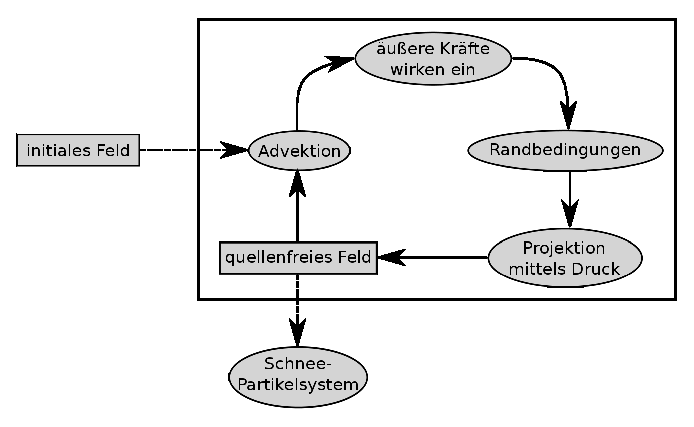
\includegraphics[width=10cm]{images/stam_loop_with_projection}
\caption{Die Simulationsschleife mit Projektion.}
\end{figure}

\subsubsection{Lösung des Poissonproblems}

Um das Vektorfeld quellenfrei zu machen, muss folgende
\PimiddyBegriff{Poissongleichung} nach $p$ gelöst werden:

\begin{equation}
\PimiddyLaplace{p} = x
\end{equation}

wobei $x$ ein Skalarfeld ist. Es existieren zahlreiche Lösungsverfahren für solch
eine Gleichung. Bei der Auswahl des Verfahrens muss beachtet werden, welches
Verfahren sich gut auf der Grafikkarte umsetzen lässt und möglichst schnell eine
ausreichend gute Lösung liefert.

Es haben sich mehrere sogenannte \PimiddyBegriff{Iterationsverfahren} als
günstig herausgestellt. Verfahren dieser Art beginnen mit einer initialen Lösung
(beispielsweise schlicht $p=0$) und nähern sich dann in jedem Iterationsschritt
weiter der eigentlichen Lösung an.

Betrachtet man große Felder, bieten sich \PimiddyBegriff{Mehrgitterverfahren}
an. Diese wurde bereits erfolgreich auf GPUs angewendet (siehe \cite{Bolz2002},
\cite{Matthias2006}). Sie sind allerdings untrivial zu implementieren, da intern
ein zweites Iterationsverfahren benötigt wird (der sogenannte
Restriktionsoperator), sowie Methoden zum hoch- und runterskalieren von
3D-Feldern.

Simplere Iterationsverfahren sind SOR (\cite{Saltvik2006}),
Gauss-Seidel-Re"-la"-xa"-ti"-on (\cite{Stam2003}) und das
Jacobiverfahren (\cite{Crane2007}, \cite{Harris2008},
\cite{Peschel2009}). Letzteres ist besonders einfach zu
implementieren und gleichzeitig hervorragend für die GPU geeignet.

\subsubsection{Das Jacobiverfahren}

Um das Jacobi-Verfahren zu veranschaulichen, soll es zunächst im
Eindimensionalen erläutert werden. Wir betrachten also kein diskretes 3D-Gitter,
sondern eine endliche Teilmenge der ganzen Zahlen (die Gitterbreite $\Delta x$
ist also $1$). Der Laplaceoperator entspricht in diesem Fall der zweiten
Ableitung von $p$.

Für die exakte Lösung $p$ des Poissonproblems muss an jeder Stelle $i$ gelten:

\begin{equation}
\label{eq:stam_jacobi_onedimensional}
\frac{
	p_{i+1} -
	2 \cdot p_{i} +
	p_{i-1}
}
{
	(\Delta x)^2
}
=
x_i
\end{equation}

Löst man diese Gleichung nach $p_i$ auf und setzt $\Delta x = 1$ ein, erhält
man:

\begin{equation}
p_i
=
\frac{
	p_{j+1} +
	p_{j-1} -
	\cdot x_i
}
{
	2
}
\end{equation}

Der Wert $p_i$ definiert sich also durch seine direkten Nachbarn $p_{i-1},
p_{i+1}$, die Gleichung ist für sich genommen nicht aufzulösen.

Sei nun eine Anfangslösung $p^0$ gegeben, z.\,B. $p^0_i = 0$ für alle $i$.
Dann lässt sich eine neue, bessere Lösung bestimmen, indem man die Werte aus
$p^0$ als Näherungen für die Nachbarn in der exakten Lösung nimmt:

\begin{equation}
\label{eq:stam_jacobi_onedimensional_iterative_solution}
p_i^1
=
\frac{
	p_{j+1}^{0} + p_{j-1}^{0} - x_i
}
{
	2
}
\end{equation}

Im nächsten Iterationsschritt berechnet man dann $p_i^2$ mit Hilfe von $p_i^1$,
usw., bis man nahe genug an die exakte Lösung herangekommen ist. In der Praxis
sind mindestens 20 Iterationen nötig, da das Verfahren sehr langsam konvergiert.

Eine leichte Konvergenzverbesserung erreicht man, indem man die rechte Seite von
\autoref{eq:stam_jacobi_onedimensional_iterative_solution} nicht direkt als neue
Lösung nimmt, sondern zwischen der bisherigen Lösung und der neue Lösung mit
einem Gewichtungsfaktor $\omega$ interpoliert:

\begin{align}
\overline{p}_i^{n+1}
&=
\frac{
	p_{j+1}^{n} + p_{j-1}^{n} - x_i
}
{
	2
} \\
p_i^{n+1}
&=
(1-\omega) \cdot p_i^n + \omega \cdot \overline{p}_i^{n+1}
\end{align}

Dieses Verfahren wird \PimiddyBegriff{gewichtete Jacobi-Iteration} genannt. In
der Praxis hat sich ein Faktor von $\omega=\frac{2}{3}$ als günstig erwiesen.

In drei Dimensionen ergibt sich dasselbe Schema, nur mit 6 Nachbarn:

\begin{equation*}
p_{i,j,k}^{n+1}
=
\frac{
	p_{i+1,j,k}^n +
	p_{i-1,j,k}^n +
	p_{i,j+1,k}^n +
	p_{i,j-1,k}^n +
	p_{i,j,k+1}^n +
	p_{i,j-1,k-1}^n -
	x_{i,j,k}^n
}
{
	6
}
\end{equation*}

\subsubsection{Randbedingungen in Differentialgleichungen}

Auch bei der Berechnung des Drucks müssen Randbedingungen beachtet werden. Dies
betrifft einerseits den Rand der Simulation, denn dort hat nicht jede Zelle 6
Nachbarn (an den Ecken des Würfels nur 3). Außerdem muss der Druck in
Hinderniszellen so gewählt werden, dass das Fluid nicht in das Hindernis
eindringt.

Es gibt im Wesentlichen zwei Arten von Randbedingungen bei einer
Differentialgleichung (wie der Poissongleichung),
\PimiddyBegriff{Dirichlet-Randbedingungen} und
\PimiddyBegriff{Von Neumann-Randbedingungen}:

\begin{itemize}
\item
	Bei Dirichlet-Randbedingungen wird der \emph{Wert} des Feldes am Rand
	fest vorgeschrieben. Beispielsweise könnte man die Druckwerte, die über
	den Simulationsrand hinausgehen (z.\,B. $p_{-1,-1,-1}$), als $0$ annehmen.
	Dies ist gewissermaßen bei der Advektion geschehen, wo die
	Geschwindigkeit bei Hinderniszellen als $(0,0,0)$ angenommen wurde.
\item
	Bei Von Neumann-Randbedingungen schreibt man die \emph{Ableitung in
	Richtung der Normalen} an einem Punkt vor:

	\begin{equation}
	\frac{
		\partial \vec{u}
	}
	{
		\partial \vec{n}
	}(x)
	=
	f(x)
	\end{equation}

	Beispielsweise könnte man $f(x)=0$ wählen. Wie bereits in
	\autoref{sec:mathematics_incompressibility_condition_section} erläutert
	bedeutet das, dass die Geschwindigkeitspfeile nicht in ein Hindernis
	hinein- oder hinauszeigen dürfen. Das Fluid darf sich aber tangential
	frei bewegen. Diese Randbedingung wird deshalb auch spezieller als
	\PimiddyBegriff{free-slip}-Randbedingung bezeichnet.
\end{itemize}

\begin{figure}[ht]
\centering
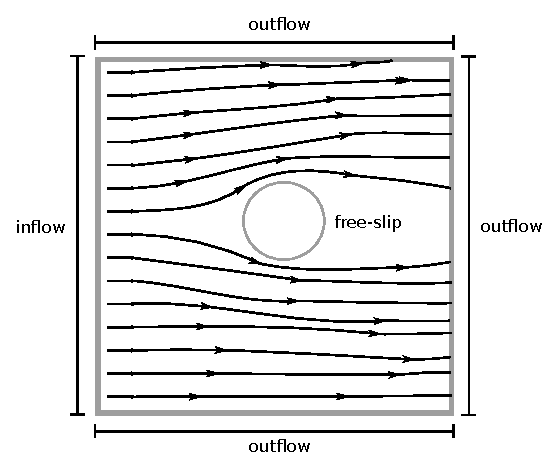
\includegraphics[width=8cm]{images/boundary_types}
\caption{Strömungslinien einer Beispielsimulation mit 3 verschiedenen Randbedingungen.}
\label{fig:stam_boundary_types}
\end{figure}

In der Simulation soll ein Teilbereich der echten Welt simuliert werden. Der
Wind wird von einigen Seiten künstlich in die Simulation gespeist. Dies nennt
man \PimiddyBegriff{inflow boundary} und ist eine Form der
Dirichlet-Randbedingung. Aus den verbleibenden Seiten soll der Wind frei aus der
Simulation \PimiddyQuotes{herausfließen}, als würde der Simulationsbereich dort
noch weitergeführt werden. Diese Art der Randbedingung nennt man
\PimiddyBegriff{outflow boundary}.

Simuliert man Rauch oder Wasser gibt es noch weitere Arten von Randbedingungen.
Die Grenze zwischen Wasseroberfläche und Luft nennt man \PimiddyBegriff{free
surface}-Randbedingung. Um diese umzusetzen müsste man $p=0$ außerhalb
des Wassers setzen. Diese Randbedingung wird hier nicht weiter beachtet.

Eine Zusammenfassung aller Randbedingungen ist in \autoref{fig:stam_boundary_types} zu sehen.

\subsubsection{Randbedingungen in der Simulation}

Es werden zuerst die Randbedingungen für die Hindernisse betrachtet. Hier sollen
\emph{free-slip}-Bedingungen erzwungen werden. Dies soll nicht explizit
hergeleitet werden, es werden nur die Veränderungen am Jacobiverfahren
beschrieben.

Im bisher beschriebenen Jacobiverfahren betrachtet man jede Zelle $p_{i,j,k}$
des Gitters und bilden die Summe über alle Nachbarzellen. Um die Randbedingungen
einfließen zu lassen, testet man, ob die Nachbarzelle von einem Hindernis
ausgefüllt ist (hier benutzen wir das Hindernisfeld $b_{i,j,k}$, was eingangs
beschrieben wurde). Gehört die Zelle zu einem Hindernis, wird nicht der
Druckwert der \emph{Nachbarzelle} zur Summe addiert, sondern der Wert der
\emph{aktuellen Zelle} (siehe \autoref{fig:stam_modified_jacobi_algorithm}
\PimiddyTodo{Wieso kann ich hier nur auf die subfigure verweisen?}). Auf
diese Weise kommt es zu keinem Druckunterschied in Richtung eines Hindernisses,
der Gradient in dieser Richtung ist also 0.  Algorithmus
\autoref{alg:stam_modified_jacobi_algorithm} zeigt den modifizierten
Algorithmus.

\begin{algorithm}
\caption{Der modifizerte Jacobi-Algorithmus}
\begin{algorithmic}
\Function{jacobi}{$p,x$}
	\State $p' = 0$
	\Comment{Ergebnisfeld ist $p'$}
	\ForAll{$(i,j,k)$}
		\State $\textrm{sum } \gets 0$
		\ForAll{Nachbarn $(i',j',k')$ von $p_{i,j,k}$}
			\If{$b_{i',j',k'} = 1$}
				\State $\textrm{sum} \gets \textrm{sum} + p_{i,j,k}$
			\Else
				\State $\textrm{sum} \gets \textrm{sum} + p_{i',j',k'}$
			\EndIf
		\EndFor
		\State $\textrm{new} = (\textrm{sum} - x_{i,j,k})/6$
		\State $p_{i,j,k}' \gets (1-\omega) \cdot p_{i,j,k} + \omega \cdot sum$
		\Comment{Gewichtete Jacobi-Iteration}
	\EndFor
	\State \Return $p'$
\EndFunction
\end{algorithmic}
\label{alg:stam_modified_jacobi_algorithm}
\end{algorithm}

\begin{figure}[ht]
\centering
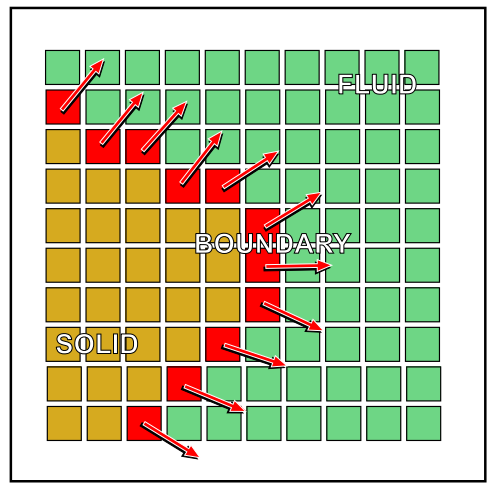
\includegraphics[width=6cm]{images/boundary_with_normals}
\caption{Hindernisse mit zugehöriger Normale}
\label{fig:stam_boundary_with_normals}
\end{figure}

Der Jacobi-Algorithmus löst die Poissongleichung allerdings nur annähernd.
Folglich werden auch die Randbedingungen nur annähernd gelöst. Dies kann im
nächsten Simulationsschritt zu Problemen führen. Daher wird in der
Implementierung die free-slip-Randbedingung nach dem Projektionsschritt
erzwungen (also nachdem der Gradient des Drucks vom Geschwindigkeitsfeld
subtrahiert wurde).

Idealerweise bräuchten wir dazu noch ein Feld $\vec{n}_{i,j,k}$, was in jedem
Punkt die Normale des Hindernisses angibt (siehe
\autoref{fig:stam_boundary_with_normals}). Dies wurde in einigen
Arbeiten umgesetzt (z.\,B. \cite{Bordignon}), es gibt jedoch eine Vereinfachung,
die dieses Feld nicht benötigt: Man iteriert erneut über alle
Gitterzellen und testet indem für jede Gitterzelle $(i,j,k)$, welche
Nachbarzellen von einem Hindernis ausgefüllt sind. Die zugehörige
Komponente der Geschwindigkeit $\vec{u}_{i,j,k}$ wird dann auf 0
gesetzt, siehe \autoref{alg:stam_enforce_free_slip}.

Für die outflow-Randbedingungen am Simulationsrand wird jede Randseite der
Simulation einzeln betrachtet. Die Geschwindigkeit einer Randzelle wird ersetzt
durch die Geschwindigkeit der \PimiddyQuotes{nächstinneren} Zelle.
Beispielsweise werden die Geschwindigkeitswerte $\vec{u}_{0,j,k}$ (also die an
der linken Simulationsseite) ersetzt durch die Werte $\vec{u}_{1,j,k}$. Analoges
wird für die anderen Seiten des Kubus getan, allerdings nicht dort, wo
inflow-Randbedingungen bestehen, wo also Wind in die Simulation hineinfließt.
Dadurch ergibt sich am Rand die Divergenz 0, der Druck ist hier also auch
annähernd 0 \PimiddyTodo{stimmt das überhaupt?}.

\begin{figure}[ht]
	\begin{subfigure}[b]{0.5\textwidth}
		\centering
		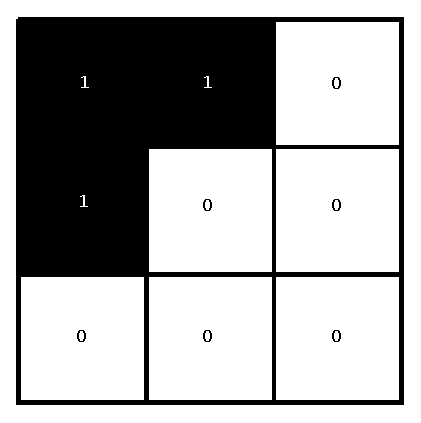
\includegraphics[width=\textwidth]{images/boundary_field_for_pressure}
		\caption{Ein beispielhaftes Hindernisfeld $b_{i,j}$}
	\end{subfigure}
	~
	\begin{subfigure}[b]{0.5\textwidth}
		\centering
		\def\svgwidth{\textwidth}
		\input{images/pressure_boundary.eps_tex}
		\caption{Die in die Druckberechnungen einfließenden Werte.}
	\label{fig:stam_modified_jacobi_algorithm}
	\end{subfigure}
\end{figure}

\begin{algorithm}
\caption{Die abschließende Randbedingungserzwingung}
\begin{algorithmic}
\Function{FreeSlipBoundary}{$\vec{v},b$}
	\ForAll{$(i,j,k)$}
		\If{$b_{i-1,j,k} = 1$ or $b_{i+1,j,k} = 1$}
			\State $\vec{u}_{i,j,k}^x = 0$
		\EndIf
		\If{$b_{i,j-1,k} = 1$ or $b_{i,j+1,k} = 1$}
			\State $\vec{u}_{i,j,k}^y = 0$
		\EndIf
		\If{$b_{i,j,k+1} = 1$ or $b_{i,j,k-1} = 1$}
			\State $\vec{u}_{i,j,k}^z = 0$
		\EndIf
	\EndFor
\EndFunction
\end{algorithmic}
\label{alg:stam_enforce_free_slip}
\end{algorithm}

\section{Implementation}

\subsection{Einleitung}

In diesem Kapitel soll auf die Details der Implementierung eingegangen werden. Es
wird zunächst OpenGL eingeführt, was zur Visualisierung eingesetzt wird. Danach
wird OpenCL eingeführt, was für die eigentlichen Berechnungen zuständig ist.

Danach das Verfahren von Stam mittels OpenCL umgesetzt. Als Ausgabe erhält man
ein Schnee-Vektorfeld, was dann weiterverwendet werden kann. Hier wird auch auf
Hindernisse wie Gebäude eingegangen. Dazu gehört das Laden der Hindernisse aus
obj-Dateien sowie die Anzeige mittels OpenGL, sowie die Einspeisung in die
Simulation.

Anschließend wird der fallende Schnee modelliert. Hierzu soll zunächst die
Entstehung von Schnee in der Natur erläutert werden, sowie physikalische
Hindergründe bezüglich fallendem Schnee.

Diese idealen physikalischen Gegebenheiten werden dann in ein einfacheres
Modell transformiert, welches für das Partikelsystem verwendet wird. Zu diesem
Partikelsystem gehört neben der Simulation auch die Visualisierung, für die in
dieser Arbeit Pointsprites verwendet werden.

Im letzten Abschnitt wird schließlich auf die Modellierung der Schneedecke
eingegangen, wobei die Ergebnisse von Manuel Schwarz \cite{Schwarz2012} eine
tragende Rolle spielen. Außerdem werden noch einige weitere
Anwendungsmöglichkeiten der Fluidsimulation wie die Simulation von Rauch
angesprochen.

\subsection{OpenGL}

\begin{itemize}
\item Herkunft, Verwendung, Shader
\end{itemize}

\subsection{OpenCL}

\subsubsection{Einleitung}

\begin{itemize}
\item CFD ist sehr anspruchsvoll was Rechenaufwand angeht
\item Traditionellerweise hat man (für Endanwender) auf CPUs programmiert
\item CPUs haben seit kurzem immerhin mehrere Kerne, sodass OpenMP und MPI Sinn ergeben
\item Die Entwicklung zu mehreren Kernen wurde von der Stromsparüberlegung angetrieben (viele Kerne mit niedrigeren Frequenzen leisten dasselbe, sind aber energieeffizienter)
\item Dadurch außerdem kleinere, spezialisiertere Prozessoren (weniger "wasted transistors")
\item Aber GPUs haben theoretisch wesentlich mehr Rechenpower\cite{Guide2012}
\item Grade CFD ist sauschnell
\item Aber natürlich brauch man Probleme, die gut parallelisierbar sind
\item Definition Concurrency: "A software system is concurrent when it consists of more than one stream of operations that are active and can make progress at one time."
\item Definition Parallelism: "When concurrent software runs on a computer with multiple processing elements so that threads actually run simultaneously, we have parallel computation. Concurrency enabled by hardware is parallelism."
\item In diesem Abschnitt Architektur von OpenCL deutlich machen und klären welche Probleme damit gut lösbar sind.
\end{itemize}

\subsubsection{Architektur}

\begin{itemize}
\item Dezember 2008 released
\item Momentan bei Version 1.2, obwohl das noch wenige implementieren
\item Parallelisierbarkeit erklären: data parallelism und task parallelism
\item Dataparallelism: Idee ist, dass man eine Sammlung von Daten hat, die
nebenläufig upgedatet werden können. Parallelität wird nun grade dadurch
erzeugt, dass man denselben Instructionstream auf jedes Datenelement abfeuert
(nicht etwa für jedes Datenelement 'nen eigenen Thread hat, der sich beliebig
 anders verhält als der nächste Thread). Beispiel: Addition zweier Vektoren
(SIMD allgemein).
\item Taskparallelism: Eignet sich vielleicht eher für Traversierung von Graphen
oder so.
\item Platform-Model erklären
	\begin{itemize}
		\item "High level description of the heterogenous system"
		\item Host (gibt nur einen)
		\item Host enthält Devices
		\item Devices enthalten Compute Units
		\item Compute Units enthalten Processing Elements
		\item Host program, was auf Host läuft
		\item Mehrere Kernel laufen auf jeweils einem Device
		\item Execution Model klärt, wie Kernel ausgeführt werden
	\end{itemize}
\item Execution-Model
	\begin{itemize}
		\item "abstract representation of how streams of instructions execute on the heterogenous platform"
		\item Kernelexecution löst die Erstellung eines ganzzahligen "Gitters" aus, jeder Kernel kriegt eine Gitterzelle, die globale ID und wird zum "Work-Item"
		\item Workitems werden in Workgroups zusammengefasst (haben auch ID, bilden eine gröbere Struktur, haben geteilten Speicher, werden auf derselben Computeunit ausgeführt)
		\item Command-Queues, schedulen Kernel, Memorycommands, Synchronisierungskommandos, in-order, out-of-order
		\item Barrieren, Warps
	\end{itemize}
\item Memory-Model
	\begin{itemize}
		\item "the collection of memory regions withing OpenCL and how they interact during an OpenCL computation"
		\item Bufferobjects (eindimensional, beliebige Datentypen), Imageobjects, mehrdimensional usw., Inhalt "versteckt"
		\item Host memory
		\item Global, local, private, constant
		\item Zusammenspiel mit OpenGL
	\end{itemize}
\item Programming model
\begin{itemize}
	\item High level abstractions for algorithm programming
	\item OpenCL-C erläutern
\end{itemize}
\end{itemize}

\subsection{Windsimulation}

\subsubsection{Allgemeines}

Für die Simulation des Winds ist es wichtig, eine möglichst optimale
Datenstruktur zur Speicherung der verwendeten Felder zu verwenden, um
die Speicherzugriffszeiten zu minimieren und die maximale Performance zu
erreichen.

Wie bereits angesprochen bietet OpenCL zur Speicherung die Wahl zwischen Buffern
und Texturen (sofern Texturen auf der Zielplattform unterstützt werden). Beide
Speicher-Arten haben leicht unterschiedliche Anwendungsgebiete. In vielen
Kerneln sind wir daran interessiert, für die \PimiddyQuotes{aktuelle} Zelle den
Wert des Gitters sowie den Wert aller Nachbarn zu bestimmen, wobei der
\PimiddyQuotes{Wert} je nach Feld-Typ entweder Druck, Geschwindigkeit oder etwas
anderes bedeuten kann. Außerdem wird bei der Advektion linear zwischen Voxeln
interpoliert.

Schnelle Zugriffe auf einen Voxel samt seiner Nachbarn sind ein Merkmal von
Texturen, daher würden sie sich für viele Kernel anbieten. Allerdings ist das
Schreiben von 3D-Texturen in OpenCL-1.1 nur mit einer Extension möglich. Als
Hilfsmaßnahme greift man hier üblicherweise zu sogenannten
\PimiddyBegriff{Flat-3D-Texturen} \cite{Harris2003}. Hier werden die einzelnen
\PimiddyQuotes{Scheiben} der dreidimensionalen Struktur nebeneinander in eine
zweidimensionale Textur geschrieben, siehe
\autoref{fig:implementation_flat_3d_texture}. Für die Umrechung zwischen 3D- und
2D-Koordinaten ist etwas Rechenaufwand nötig. 2D-Texturen erlauben außerdem
natürlicherweise nur zweidimensionale Interpolation. Benötigt man
dreidimensionale Interpolation, ist auch hier etwas Mehraufwand zu verrechnen.
Texturen werden optimiert gespeichert, sodass Leseoperationen beschleunigt
werden. Diese optimierte Speicherung führt aber dazu, dass das Schreiben in
Texturen relativ langsam ist. Benchmarks im Zweidimensionalen bestätigten, dass
Buffer tatsächlich schneller sind.

\begin{figure}[ht]
\centering
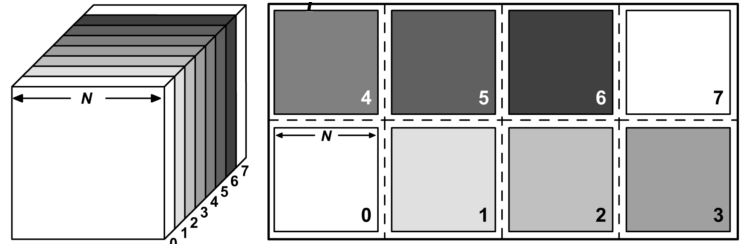
\includegraphics[width=10cm]{images/flat_3d_texture}
\caption{Veranschaulichung einer Flat-3D-Textur}
\label{fig:implementation_flat_3d_texture}
\end{figure}

Da Buffer eindimensional sind, muss zwischen drei- und eindimensionalen
Koordinaten konvertiert werden. Sei $(x,y,z)$ eine dreidimensionale Koordinate
und $(w,h,d)$ die Dimensionen eines Buffers (er enthält also $w \cdot h \cdot d$
Elemente). Dann erhält man den eindimensionalen Index mittels:

\begin{equation}
i = w \cdot h \cdot z + w \cdot y + x
\end{equation}

Umgekehrt erhält man die $(x,y,z)$-Koordinaten eines Index mittels

\begin{align*}
x &= i \PimiddyModulo w \\
y &= i \PimiddyModulo w \cdot h \\
z &= i / (w \cdot h)  \\
\end{align*}

Im Weiteren wird das Verfahren von Stam in OpenCL umgesetzt. Dabei wird auf
Besonderheiten in der Implementierung eingegangen. Fast alle Kernel greifen
hierbei auf den Buffer zurück, der die Hindernisinformationen enthält. Wie
dieser Buffer gefüllt wird, wird im letzten Abschnitt erläutert.

\subsubsection{Verfahren nach Stam in OpenCL}

Es sollen nun die einzelnen Schritte des Verfahrens in OpenCL-Kernel umgewandelt
werden, wobei an einigen Stellen auf Details verzichtet wird. Der Teil des
Programms, der auf dem Host läuft, soll hier ebenfalls nicht in Gänze erarbeitet
werden. Stattdessen soll deutlich werden, in welcher Reihenfolge die Kernel
aufgerufen werden und welche Daten beim Aufruf gelesen und geschrieben werden.
Aus Einrückungsgründen werden viele Bezeichner abgekürzt, aber immer so, dass aus
der Erläuterung bzw. den Kommentaren noch hervorgeht, was sich dahinter
verbirgt.

Die Simulation benötigt einige persistente Daten Daten, also solche, die
zwischen den Simulationsschritten beibehalten werden und nicht nur temporär für
berechnungen verwendet werden:

\begin{itemize}
\item ein Buffer \PimiddyInlineCode{boundaries} vom Typ
\PimiddyInlineCode{float}, der 1.0 enthält, wenn die zugehörige Gitterzelle ein
Hindernis enthält und 0.0 wenn nicht. Das Befüllen dieses Buffers wird in
Abschnitt xxx beschrieben.
\item ein Buffer \PimiddyInlineCode{velocity} vom Typ
\PimiddyInlineCode{float4}, der das momentane Geschwindigkeitsfeld enthält.
Dieses Feld wird anfangs auf $(0,0,0,0)$ gesetzt. Der Wind wird manuell von
einer Seite in die Simulation gespeist und breitet sich dann aus.
\item Viele der Algorithmen benötigen außerdem das aktuelle Zeitdelta
\PimiddyInlineCode{float dt}, was die Zeit seit dem letzten Simulationsdurchlauf
angibt.
\end{itemize}

Die meisten Kernel werden mit einer dreidimensionalen Arbeitsgröße initialisiert
und müssen auf den aktuellen Voxel, sowie seine Nachbarn zugreifen. Daher bietet
es sich an, den Übergang von einem drei- zu einem eindimensionalen Index in eine
Funktion auszulagern. Diese Funktion kann gleichzeitig testen, ob ein gegebener
Index den Rand des Gitters verlässt, und in dem Fall den nächstbesseren Voxel am
Rand zurückliefern. Diese Funktion \PimiddyInlineCode{i4p} ist im Folgenden
dargestellt:

\begin{lstlisting}
// Bekommt die Gittergroesse s und eine 3D-Position p.
// Liefert einen Index.
uint i4p(uint4 p,uint4 s)
{
	// Komponentenweise in gueltigen
	// Bereich [0,n-1] transformieren
	p = clamp(p,(uint4)(0),s - (uint4)(1));
	return s.w * s.h * p.z + s.w * p.y + p.x;
}
\end{lstlisting}

Der erste Schritt im Verfahren von Stam ist die Advektion des Vektorfeldes
\PimiddyInlineCode{velocity}. Der dazugehörige Kernel ist in mehreren Funktionen
und Strukturen aufgeteilt, die nun im einzelnen erklärt werden sollen.

Man benötigt zunächst eine Struktur, um einen Geschwindigkeitswert sowie die direkten
Nachbarn zu speichern (siehe \autoref{implementation_right_neighbors}).

\begin{figure}[ht]
\centering
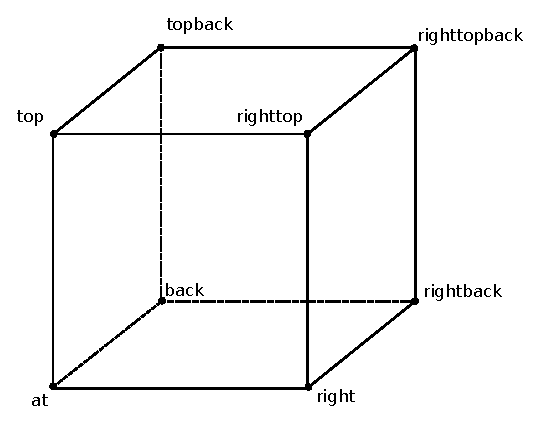
\includegraphics[width=10cm]{images/right_neighborhood}
\caption{Veranschaulichung der Nachbarschaftsstruktur \PimiddyInlineCode{neighbors}}
\label{fig:implementation_right_neighbors}
\end{figure}

\begin{lstlisting}
typedef struct neighbors
{
	float4 at;
	float4 right,top,back,righttop;
	float4 rightback,topback;
	float4 righttopback;
};
\end{lstlisting}

Diese Struktur wird von einer zugehörigen Funktion zurückgegeben, die eine
beliebige Position im Gitter sowie die Größe des Gitters als Eingabe bekommt:

\begin{lstlisting}
// Parameter genau wie i4p, zusaetzlich
// noch "b"
neighbors neighbors_for_pos(
	global float4 *b,
	uint4 p,
	uint4 s)
{
	neighbors result;
	result.at = b[i4p(p,s)];
	result.right = b[i4p(p+(uint4)(1,0,0,0),s)];
	result.top = b[i4p(p+(uint4)(0,1,0,0),s)];
	result.back = b[i4p(p+(uint4)(0,0,1,0),s)];
	result.righttop = b[i4p(p+(uint4)(0,1,1,0),s)];
	result.rightback = b[i4p(p+(uint4)(1,0,1,0),s)];
	result.topback = b[i4p(p+(uint4)(0,1,1,0),s)];
	result.righttopback = b[i4p(p+(uint4)(1,1,1,0),s)];
	return result;
}
\end{lstlisting}

Schließlich wollen wir mit Hilfe dieser Nachbarstruktur einen interpolierten
Vektor erzeugen. Hier hilft die Funktion \PimiddyInlineCode{mix}, die linear
zwischen zwei Werten anhand eines dritten Wertes interpoliert:

\begin{lstlisting}
float4 interpolate_neighbors(
	neighbors n,
	// v ist ein Vektor im Intervall [0 ,1]
	float4 v)
{
	float4
		v1 =
		mix(
			mix(n.at ,n.right ,v.x),
			mix (n.top ,n.righttop ,v.x),
			v.y),
		v2 =
		mix(
			mix(n.back ,n.rightback ,v.x),
			mix(n.topback ,n. righttopback ,v.x),
			v.y);

	return mix(v1,v2,v.z);
}
\end{lstlisting}

Der eigentliche Kernel hat schließlich folgende Form:

\begin{lstlisting}
kernel void advection(
	global float *boundary,
	global float4 *input,
	global float4 *output,
	float dt,
	uint4 size)
{
	uint4 position = (int4)(
		get_global_id(0),
		get_global_id(1),
		get_global_id(2),
		0);

	uint index = i4p(position);

	if(boundary[index] > 0.5f)
	{
		output[index] = (float4)(0.0f);
		return;
	}

	float4
		v = input[index],
		advected = convert_float4(position) - dt * v,
		fractions = fract(advected_vector);

	neighbors n = neighbors_for_pos(
		input,
		position,
		size);

	output[index] = interpolate_neighbors(
		n,
		fractions);
}
\end{lstlisting}

ür den Projektionsschritt benötigen wir die Divergenz des Vektorfeldes.
Analog zur Advektion definieren wir eine Struktur, um die Von Neumann-
Nachbarschaft eines Gitterpunktes zu speichern:

\begin{lstlisting}
typedef struct vn_neighbors
{
float4 at;
float4 left , right;
float4 top ,bottom ;
float4 front , back ;
float boundary_at ;
float boundary_left , boundary_right ;
float boundary_top , boundary_bottom ;
float boundary_front , boundary_back ;
};
\end{lstlisting}

Die Struktur enthält zusätzlich noch die zu den Nachbarn gehörigen Hin-
derniswerte, die Bestimmung dieser Werte und die der Vektoren verläuft aber
nach demselben Schema wie bei der Advektion und sei im Folgenden mit
vn_neighbors_for_pos(...) bezeichnet.
Bei der Bestimmung der Divergenz müssen die Randbedingungen beachtet
werden. Ist einer der Nachbarn von einem Hindernis ausgefüllt, wird statt des
Vektors an dieser Stelle der Nullvektor angenommen. Statt dies jedoch als eine
womöglich aufwändige Bedingung umzusetzen kann stattdessen erneut dieFunktion mix verwendet werden, wobei als Interpolationsparameter direkt der
Hinderniswert eingesetzt wird. Der zur Divergenz gehörige Kernel sieht so
aus:

\begin{lstlisting}
kernel void divergence (
global float4 *input ,
global float *output ,
global float * boundary ,
uint4 size )
{
uint4 position = (int4 )(
get_global_id (0),
get_global_id (1),
get_global_id (2),
0);
uint index = i4p ( position );
vn_neighbors n = vn_neighbors_for_pos (
input ,
position ,
boundary ,
size );
float4 z = ( float4 )(0.0f);
n. left = mix (n.left ,z,n. boundary_left );
n. right = mix (n.right ,z,n. boundary_right );
n.top = mix (n.top ,z,n. boundary_top );
n. bottom = mix (n.bottom ,z,n. boundary_bottom );
n. front = mix (n.front ,z,n. boundary_front );
n. back = mix (n.back ,z,n. boundary_back );
output [ index] =
(n.right - n.left ).x +
(n.bottom - n.top ).y +
(n.front - n.back ).z;
}
\end{lstlisting}

\begin{itemize}
\item Erklärung der Algorithmen mit (Pseudo?)-Code
\item Zuerst Advektion. Hier ansprechen, dass vielleicht Texturen besser wären
wegen "random gather" und Interpolation, aber dazu Umkonvertierung
\item Dann Jacobiverfahren, hier vor allem Pingpong zwischen Buffern erklären
und wie viele Iterationen man machen muss/kann.
\item Dann Subtraktion des Gradienten
\item Hindernisse, Visualisierung (Laden aus obj-Datei)
\item Hindernisse, Voxelisierung mit binvox (Quelle \cite{Nooruddin2003}, \cite{binvox2012}
\end{itemize}

\subsection{Fliegender Schnee}

\begin{itemize}
\item Grundsätzliche Einteilung
	\begin{itemize}
	\item Kurze Einführung wo Schnee herkommt
	\item Aussehen der Schneeflocken
	\item Simulation der Schneeflocken, erst Physikalisch
	\item Dann, wenn nötige Eigenschaften bekannt sind, Partikelsystem erklären
	\end{itemize}
\item Niederschlag erklären: Luft im Himmel ist mit Wasser gesättigt, das
gesättigte Wasser kondensiert zu Tropfen, Tropfen wachsen bis sie
herunterfallen. Tropfen bilden sich nur, wenn Kondensationskerne (wie Staub) in
der Luft sind, an die das Wasser sich anheften kann.
\item Schneefall: Temparatur muss kleiner 0 Grad sein. Kondensationskerne müssen
eine gewisse Form haben (wird bei $<-40$ Grad unnötig)
\item Schneeflocken haben sehr vielfältige Formen und Größen (Entstehung dieser Formen kurz erklären?)
\item Werden visuell vereinfacht zu Point Sprites
\item Point Sprites Punkte mit Ausdehnung und Textur, zeigen immer zum
Betrachter, Größe selber festlegbar, abhängig von der Kamera, Bild wird atlased
und je nach Flockeneigenschaft (bzw. Temparatur der Umgebung) ausgewählt
\item Physikalische Eigenschaften einer Schneeflocke
\item Kräfte sind gravity, buoyant, lift und drag.
\item Drag ist die Kraft, die die Schneeflocke entlang des Wind treiben lässt
\item Lift lässt die Flocke in Kreisförmigen Bewegungen runterfallen
\item Drag ist definiert durch
\[
F_{drag} = \frac{1}{2} \rho_{air} \vec{U}_{fluid}^2 A C_D
\]
wobei $\rho$ die Dichte der Luft angibt, $U$ die
Geschwindigkeit, $A$ der Durchmesser, $C_D$ der Drag-Koeffizient, der auf die
Form der Schneeflocke ankommt und die Turbulenzen die sie erzeugt.
\item Angenommen die Schneeflocke hat eine bestimmte Masse und fällt mit
terminal velocity nach unten, dann kann man $C_D$ bestimmen (abhängig von $U_{max}, \rho, A, m_{snow}$
\item Das kann man in $F_{drag}$ einsetzen und erhält
\[
F_{drag} = \frac{U_{fluid} m_{snow} g}{U_{max}}
\]
\item Man muss also nur $U_{max}$ schätzen. In \cite{Hanesch1966} wurde das
gemacht (bei -2 bis 0 Grad Celsius). Feststellung: Größe der Schneeflocke hat
kaum Einfluss. Geschwindigkeit ist zwischen $0.5m/s$ und $2m/s$. In
\cite{Canada1999} wurde zudem festgestellt, dass zwischen trockenem Schnee und
nassem Schnee ein Faktor von 2 ergibt, d.h. nasser Schnee hat $1-4m/s$ und
trockener eben $0.5-2$
\item Lift force ist orthogonal zur Dragforce und entsteht durch vortex shedding
hinter der Schneeflocke. Flocke wird zur Seite abgetrieben.
\item Via Weg-Zeit-Gesetz:
\[
s=\frac{1}{2}at^2 + v_0 t + s_0
\]
Berechnen wir die neue Position eine Schneeflocke via:
\[
\vec{p}^{t+\Delta t} = \vec{p}^t + \vec{u} \Delta t + \frac{1}{2} \vec{a} \Delta t^2
\]
D.h. wir speichern eine Geschwindigkeit und Berechnen eine (konstante) Beschleunigung

\textbf{Alternativ}: Schlicht zwei DGL hinschreiben:
\begin{gather}
p^{t + \Delta t} = p^{t} + \Delta t \cdot \vec{u}^{t} \\
\vec{u}^{t+ \Delta t} = \vec{u}^{t} + \Delta t \cdot \vec{a}^{t} \\
\vec{a}^t = \frac{\vec{F}_{ges}}{m_{snow}}
\end{gather}
\item Erste Kraft, Gravitation
\item Zweite Kraft, Auftrieb, wird aber vernachlässigt
\item $F_{lift}$ erzeugt spiralförmige Bewegung, allerdings relativ subtil. Wird angenähert durch:
\[
U_{circ} = C_{vel} \omega (\sin(\omega t),0,\cos(\omega t))
\]
\item Erstmal weglassen
\item Nötige Eigenschaften einer Schneeflocke: Position, Geschwindigkeit (dynamisch), Masse (für Drag), Maximalgeschwindigkeit $U_{max}$.
\item Simulation vom Aufbau her:
	\begin{itemize}
		\item Generiere Zufallswerte für Schneeflockenposition-,
		Geschwindigkeit, Masse, Maximalgeschwindigkeit, Bild
		\item In jedem Frame update Geschwindigkeit und Position
		\item Teste auf Hindernis, falls erfolgreich, generiere neue
		Zufallsposition (oder wenn Schneeflocke außerhalb ist)
		\item Update ggf. die Schneeaktivität.
	\end{itemize}
\item Simulation in Code, Buffersharing mit OpenGL, Shader in OpenG.
\end{itemize}

\subsection{Liegengebliebener Schnee}

\begin{itemize}
\item Marching Cubes, allgemeine Beschreibung
\item Marching Cubes auf der GPU
\item Zusammenhang mit Schneemodell
\item Triplanare bzw. prozedurale Texturierung
\end{itemize}

\subsection{Andere Visualisierungsmöglichkeiten}

\begin{itemize}
\item Rauch
\end{itemize}


\bibliographystyle{plain}
\bibliography{mendeley_bibliography,other_sources}

\end{document}
